%! TEX program = LuaTeX

\documentclass[nobackground,dvipsnames,table]{beamer}
\usepackage{cs152}

\mode<presentation>
{\usetheme{Hannover}
    \usecolortheme{cs152}
    \setbeamercovered{transparent}
    \useinnertheme[shadow=false]{rounded}
    \usebackgroundtemplate{}
    \setbeamercolor*{frametitle}{parent=palette primary}
    \setbeamerfont{block title}{size={}}
    \setbeamertemplate{navigation symbols}{}
}

\title{Suicide and Self-Harm}
\subtitle{CS 152 --- Lecture 8}

\author[A. Stamos]{Alex Stamos}
\institute[Stanford University]{Stanford Cyber Policy Center}
\date[2022]{\today}
\subject{CS 152 --- Trust and Safety Engineering}
%\titlegraphic{
\includegraphics[width=5cm]{img/cyber-logo-white-black-red-WEB}}

% Change the level of bulleting on the ToC page
\setcounter{tocdepth}{2}

\graphicspath{{img/lesson08}}

\begin{document}

\begin{frame}
    \titlepage
\end{frame}

\begin{frame}{Content Warning}%TODO black background?; will need to update for other colleges because hotlines sound very Stanford-specific
    This lecture will discuss suicide and self harm. This material can be stressful or triggering for students who have experience with these issues. This is not a psychology course and will therefore approach this topic from a technical perspective.\\~\\
    If you or someone you know is in need, 24/7 support is available for students:
    \small
    \begin{itemize}
        \item CAPS at (650) 498-2336 and \url{https://vaden.stanford.edu/get-help-now}
        \item Graduate Life Office (GLO) at (650) 723-7288, pager 25085
        \item Bridge Peer Counseling Center at (650) 723-3392
        \item Stanford Confidential Support Team 24/7 hotline: +1 (650) 725-9955
        \item National Suicide Prevention Lifeline: (800) 273-8255 and \url{https://suicidepreventionlifeline.org/}
        \item The Office for Religious Life at (650) 723-1762
    \end{itemize}
\end{frame}

\section{The Molly Russell Case}

\begin{frame}{The Molly Russell Case}
    \begin{columns}
        \column{0.5\textwidth}
            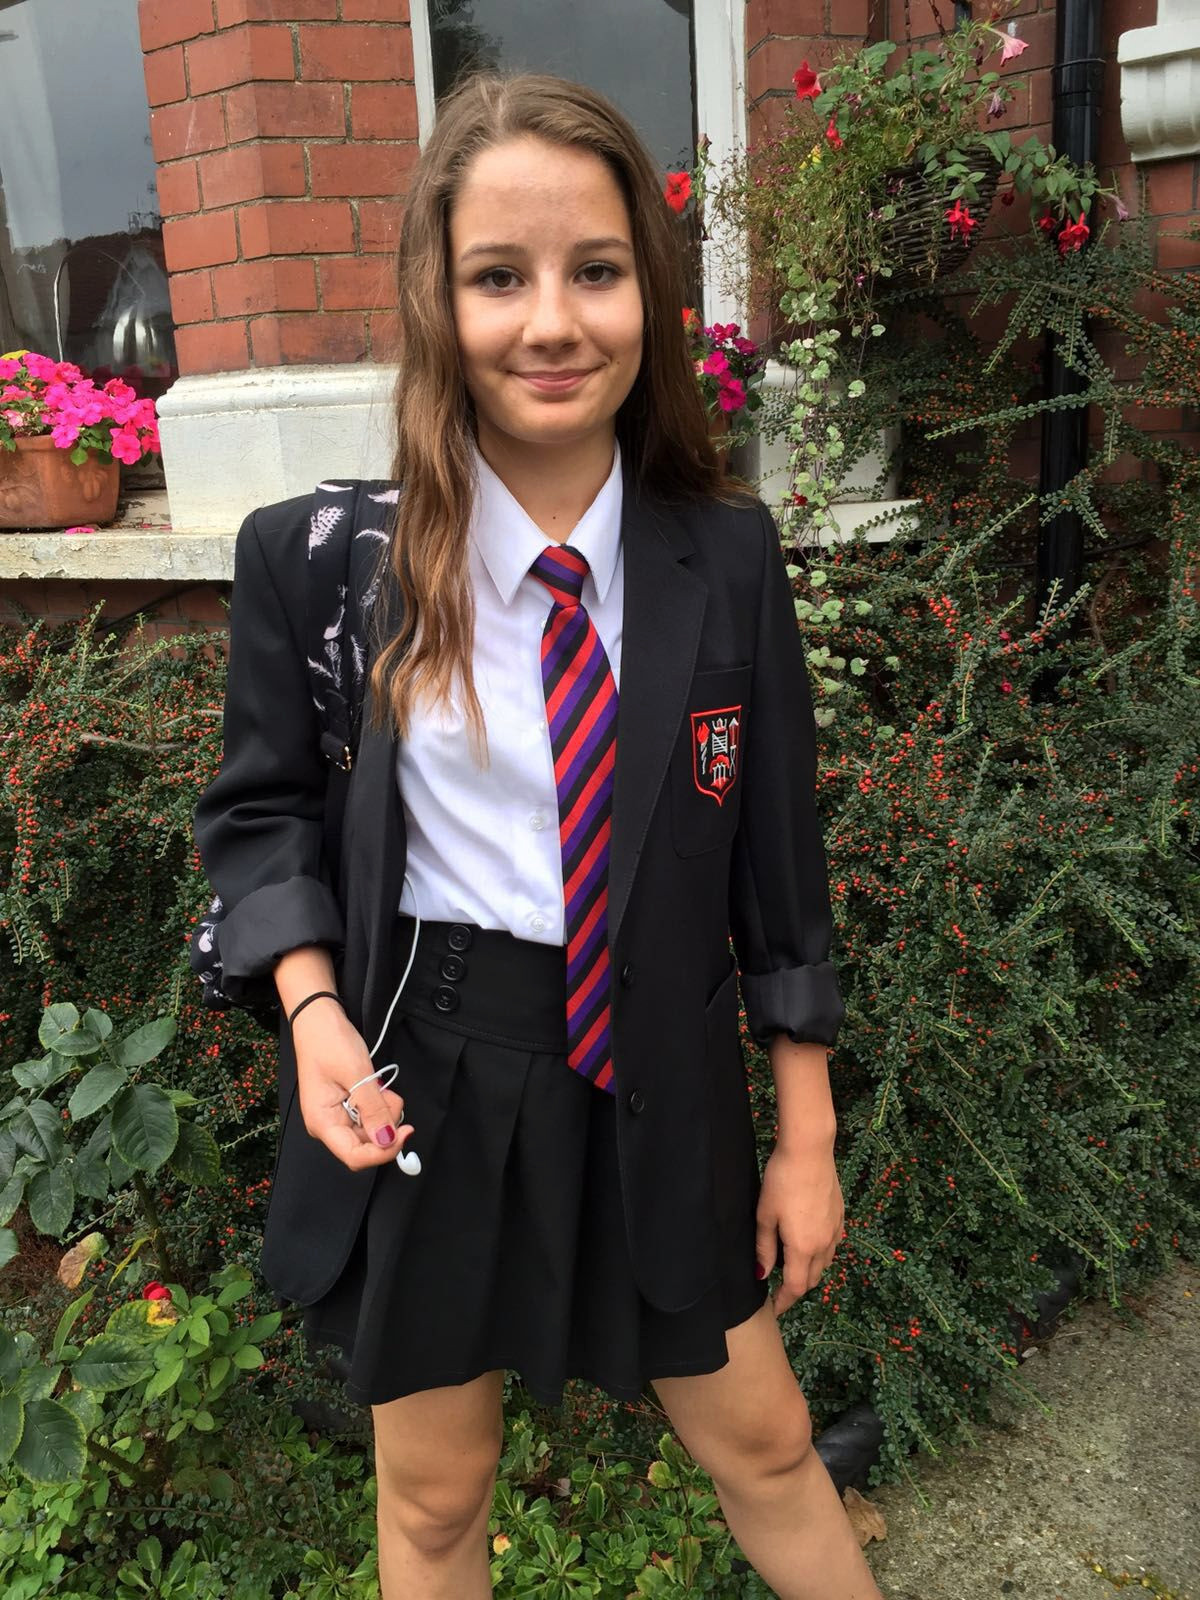
\includegraphics[width=\textwidth]{molly-russell}
        \column{0.4\textwidth}
            \centering
            \large
            “I have no doubt that Social Media helped kill my daughter”\\
            - Ian Russell
    \end{columns}
\end{frame}

\begin{frame}{The Molly Russell Case}
    \begin{columns}
        \column{0.5\textwidth}
            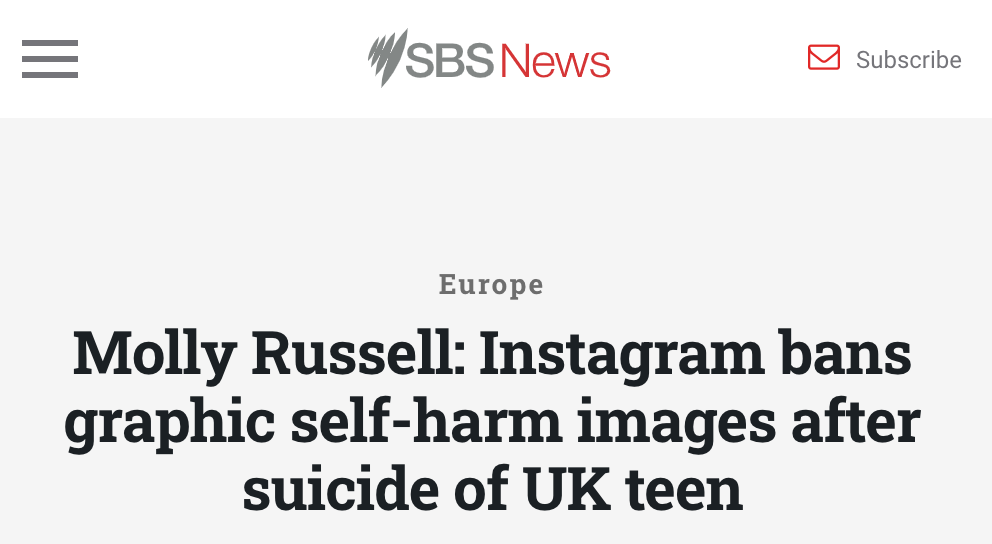
\includegraphics[width=\textwidth]{molly-russell-article-1}
            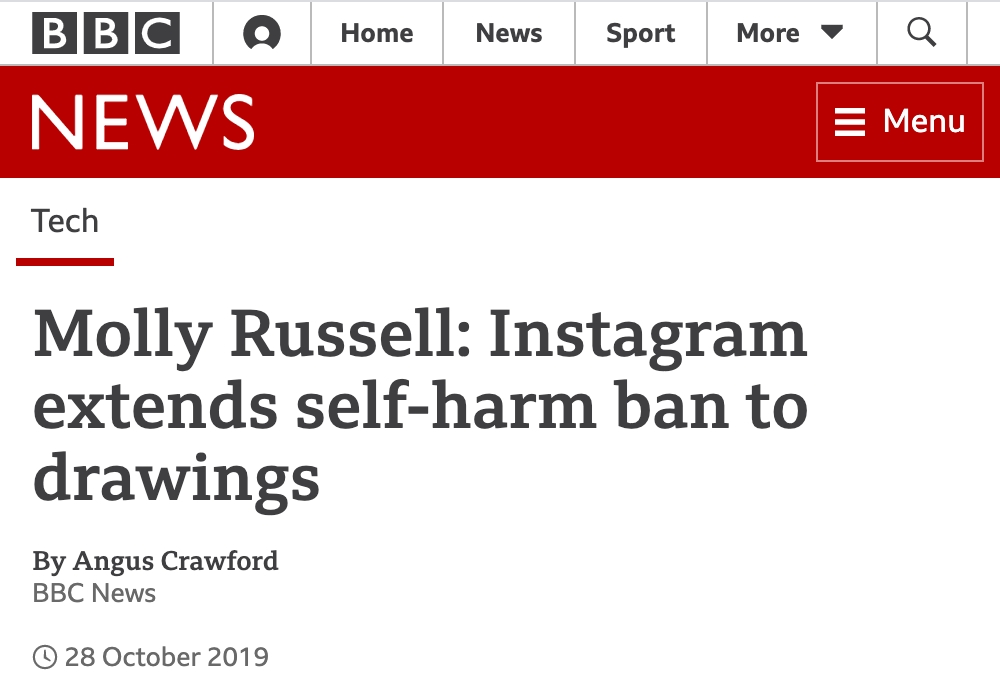
\includegraphics[width=\textwidth]{molly-russell-article-2}
        \column{0.5\textwidth}
            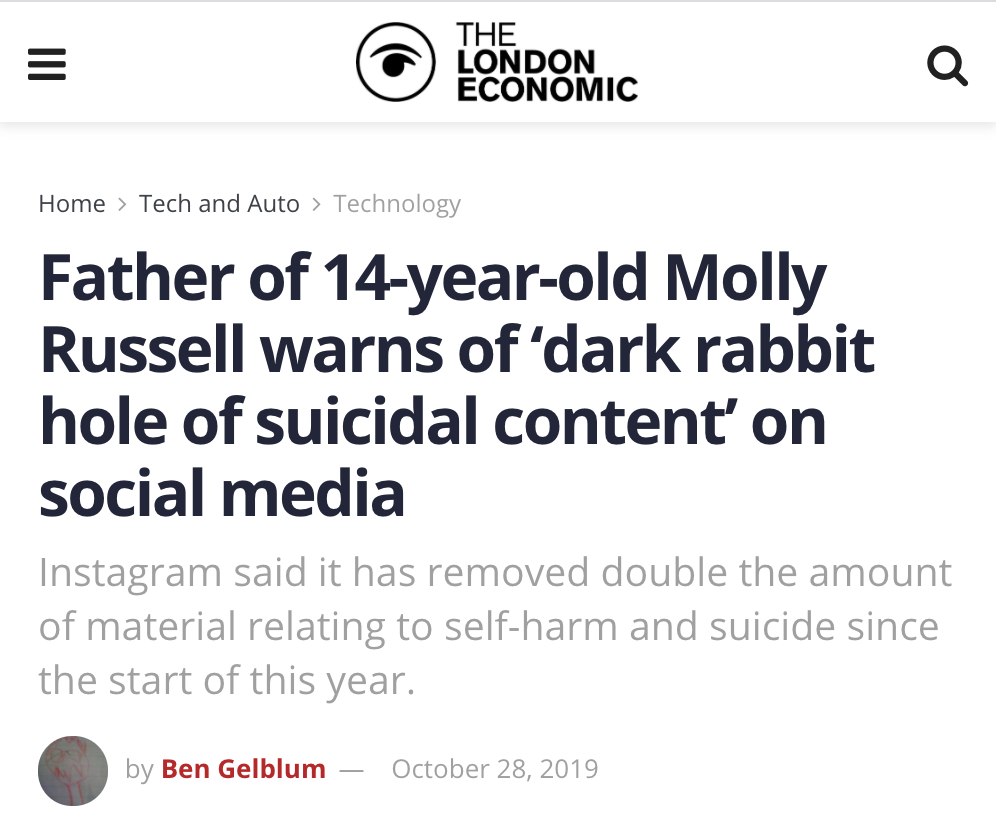
\includegraphics[width=\textwidth]{molly-russell-article-3}
            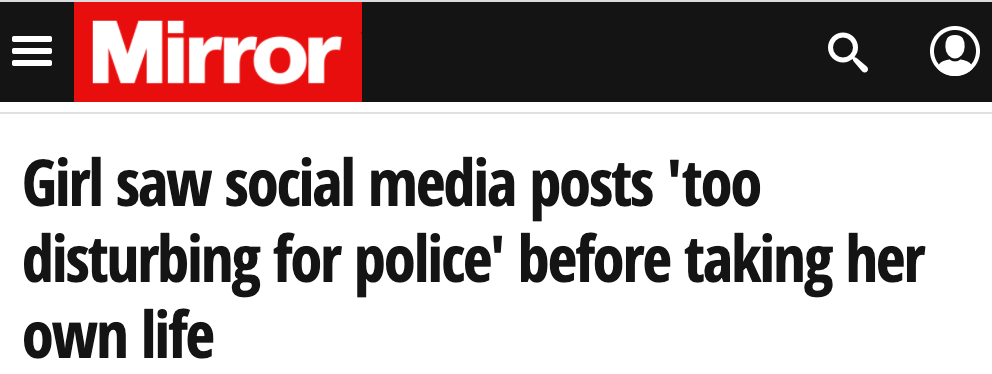
\includegraphics[width=\textwidth]{molly-russell-article-4}
    \end{columns}
\end{frame}

\begin{frame}{The Molly Russell Case}
    Instagram Policy Changes:\\
    \begin{itemize}
        \item \textbf{Sept. 2018:} published a Parent’s Guide
        \item \textbf{Feb. 2019:} banned graphic suicide and self-harm content, restricted discoverability, blocked hashtags, added sensitivity screens
        \item \textbf{Oct. 2019:} banned fictional or illustrated depictions and content containing methods
        \item \textbf{Sept. 2020:} expanded partnerships with suicide prevention NGOs
        \item \textbf{Oct. 2020:} added help messages at the top of all search results related to suicide or self-injury
    \end{itemize}
\end{frame}

%\section{\href{https://stanford.zoom.us/rec/play/aiwHhkmccXZcqagFteF7VRaxdfCZRc8yEydmuGPuaBoKy1_9p0jN8hJaduagSDUZhwhv5stNQDg7mHMp.Bb-trfbEbDy0mV6-?autoplay=true&startTime=1643760188000}{10 minute Video interview with Dr. Anna Van Meter}}%TODO is this still relevant this year?

\section{Self-Harm Overview}%TODO better section title?

\begin{frame}{Why Cover Self-Harm in This Class?}
    \large
    \begin{itemize}
        \item Detecting cries for help
        \item Incitement to self harm or suicide
        \item Support communities
        \item Do platforms have a moral imperative to act?
    \end{itemize}
\end{frame}

\begin{frame}{}
    \begin{columns}
        \column{0.55\textwidth}
            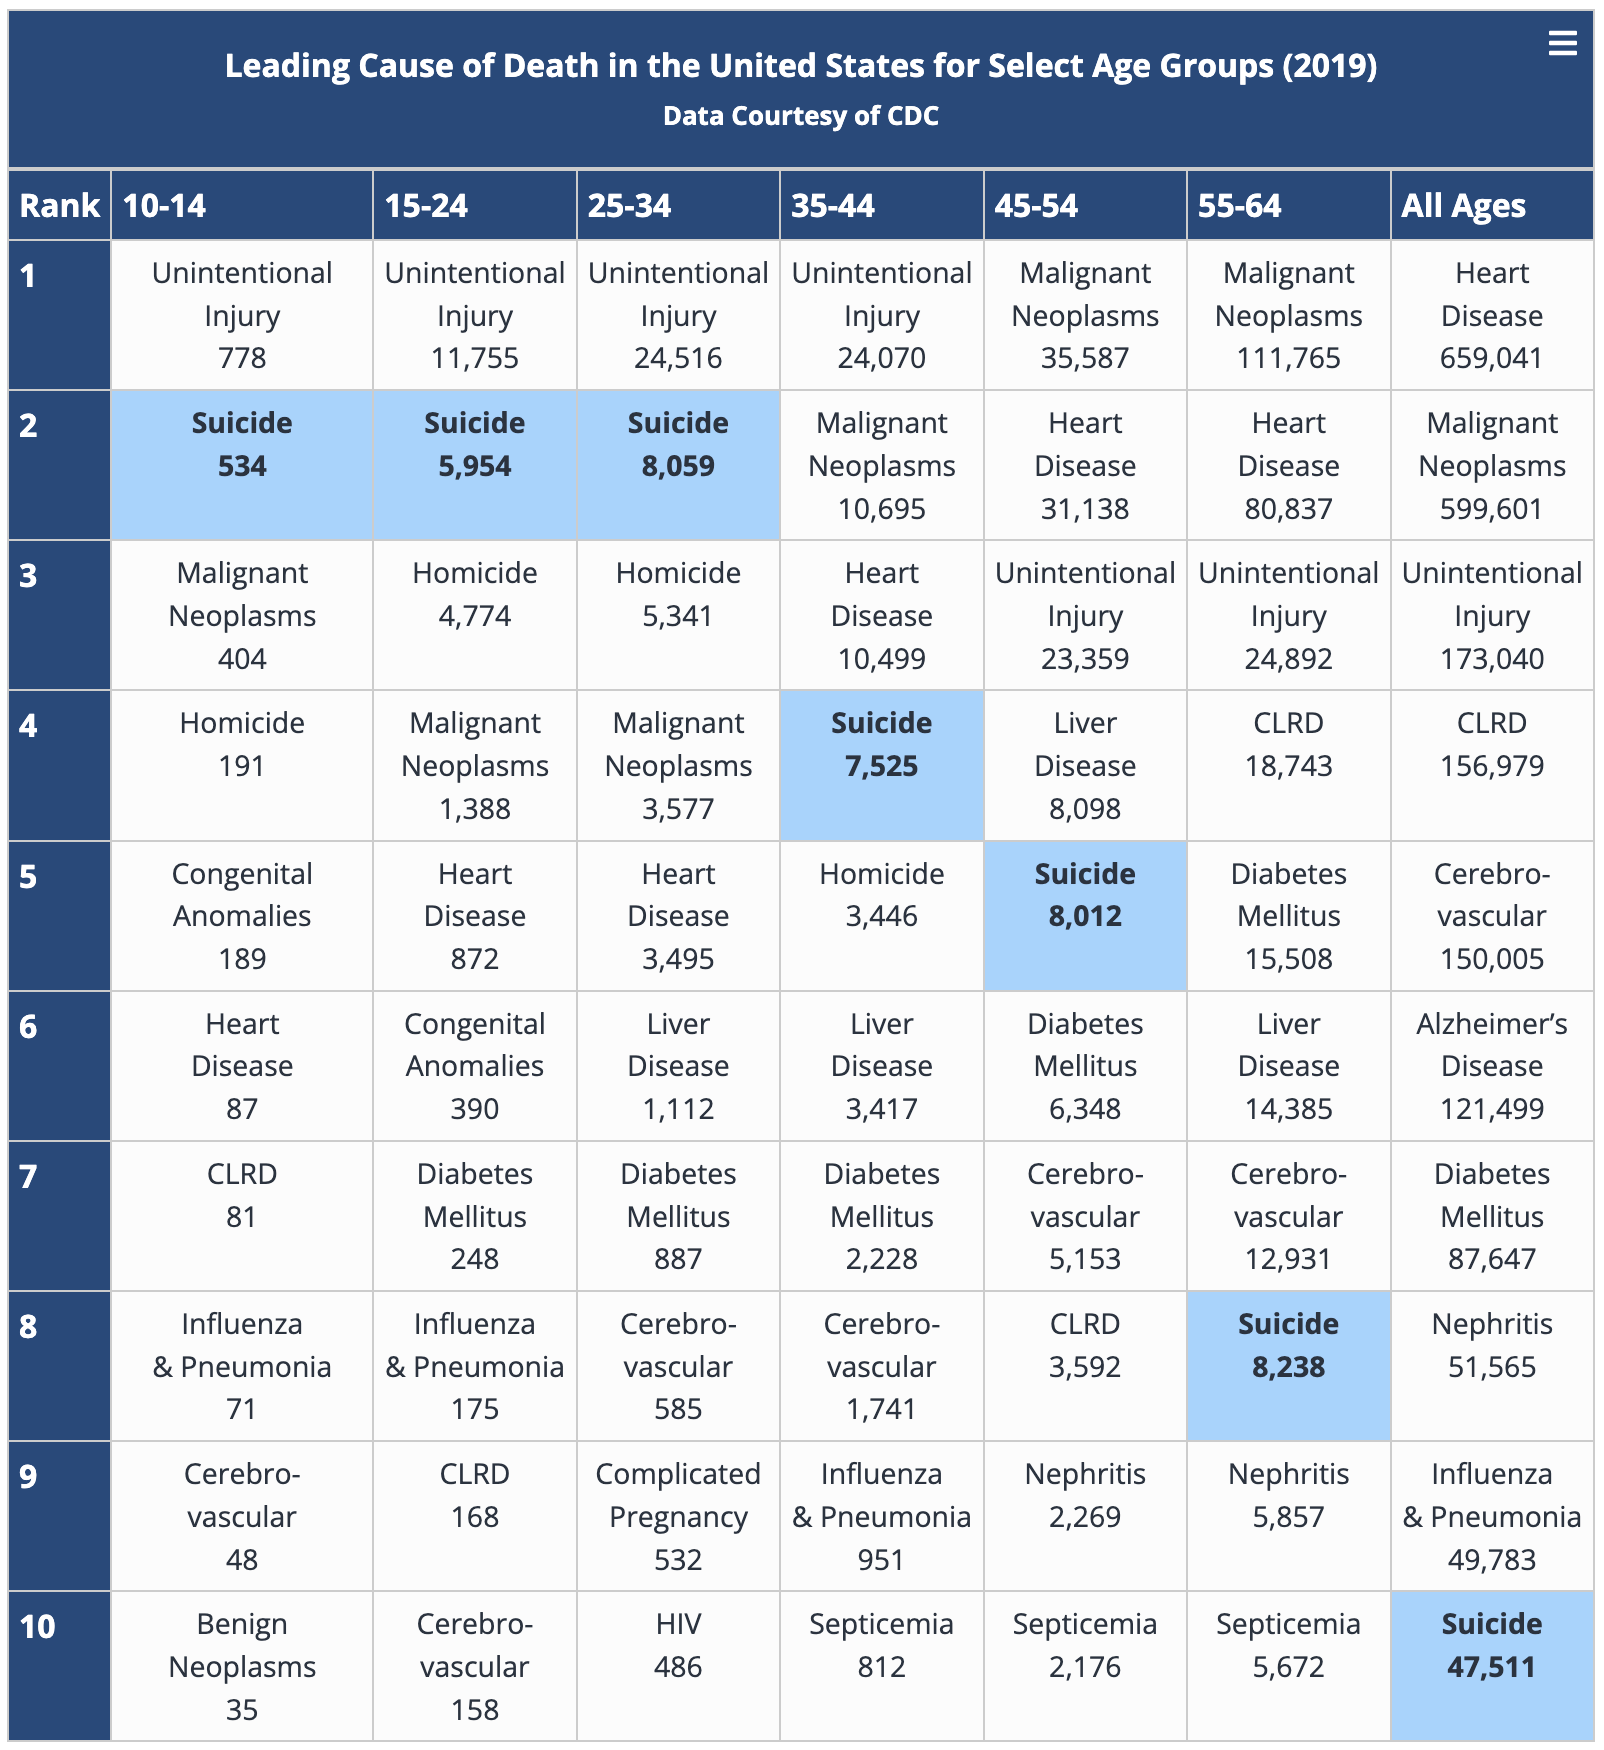
\includegraphics[width=\textwidth]{leading-causes-of-death-suicide-2019}
            \tiny
            \url{https://www.nimh.nih.gov/health/statistics/suicide}
        \column{0.45\textwidth}
            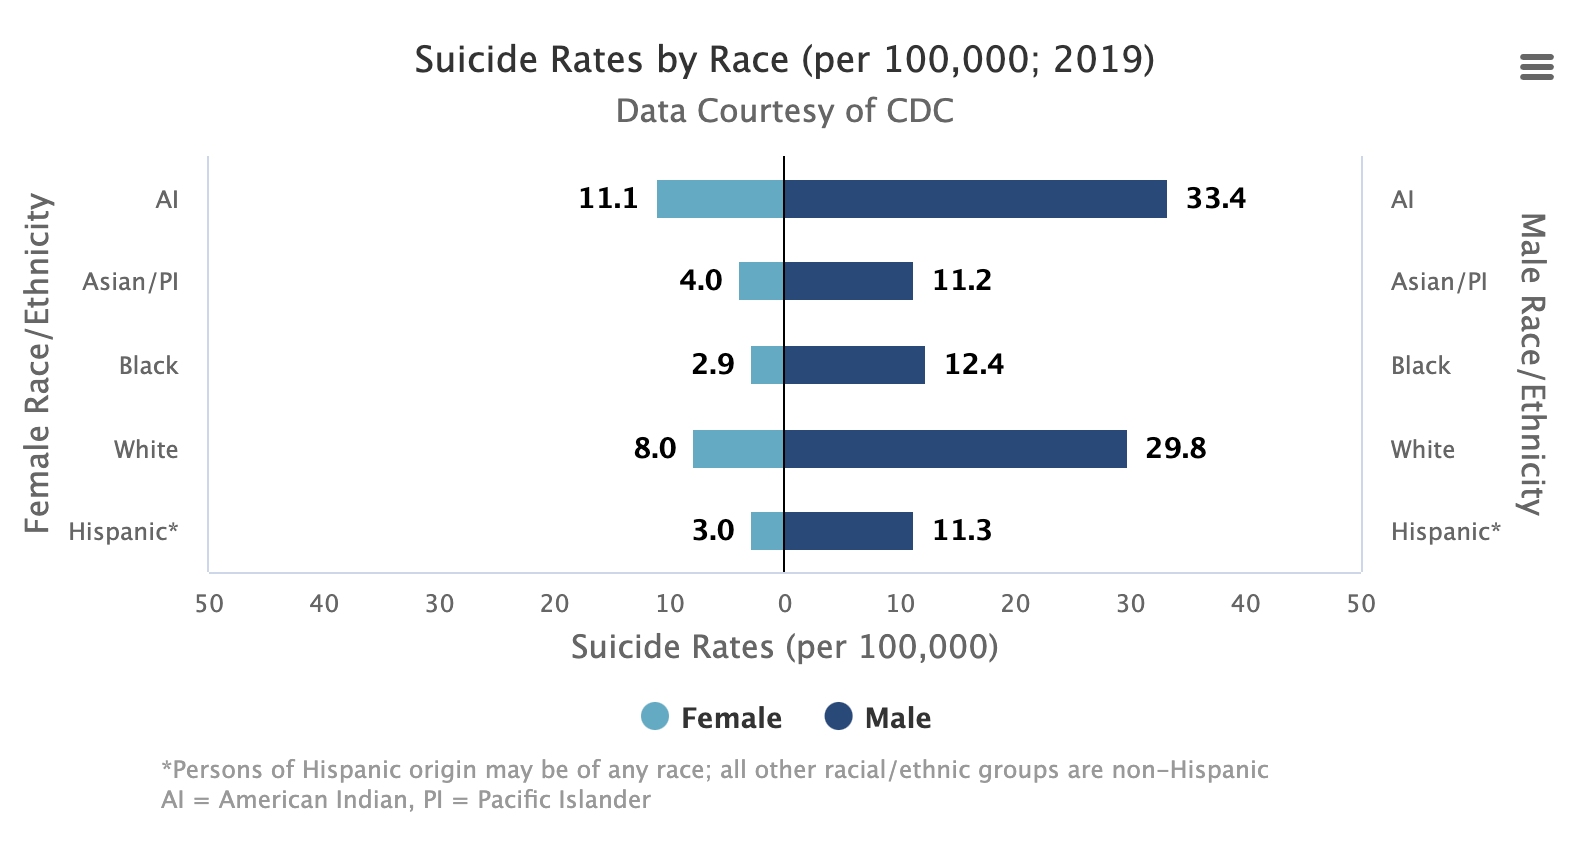
\includegraphics[width=\textwidth]{suicide-rates-by-race}
    \end{columns}
\end{frame}

\begin{frame}{How Does Self-Harm Manifest on Platforms?}
    \begin{columns}
        \column{0.5\textwidth}
            \footnotesize
            \begin{itemize}
                \item Images and instructions
                \item Live video depictions
                \item ‘Inspiration’ content or glorification
                \item Inciting harassment or bullying
                \item Suggested searches
                \item Normalization 
                \item Sensationalization/ broad coverage of specific incidents
                \item Targeted Ads
                \item Communities that validate or encourage harmful behavior
                \item Survivor photos / support communities
                \item \textit{Usually excluded from policies:}
                \begin{itemize}
                    \footnotesize
                    \item \textit{Substance abuse}
                    \item \textit{Health and wellness misinfo}
                \end{itemize}
            \end{itemize}
        \column{0.5\textwidth}
            
\includegraphics[width=\textwidth]{message-to-instagram}
    \end{columns}
\end{frame}

\begin{frame}{Context Matters}
    \begin{columns}[T]
        \column{0.5\textwidth}
            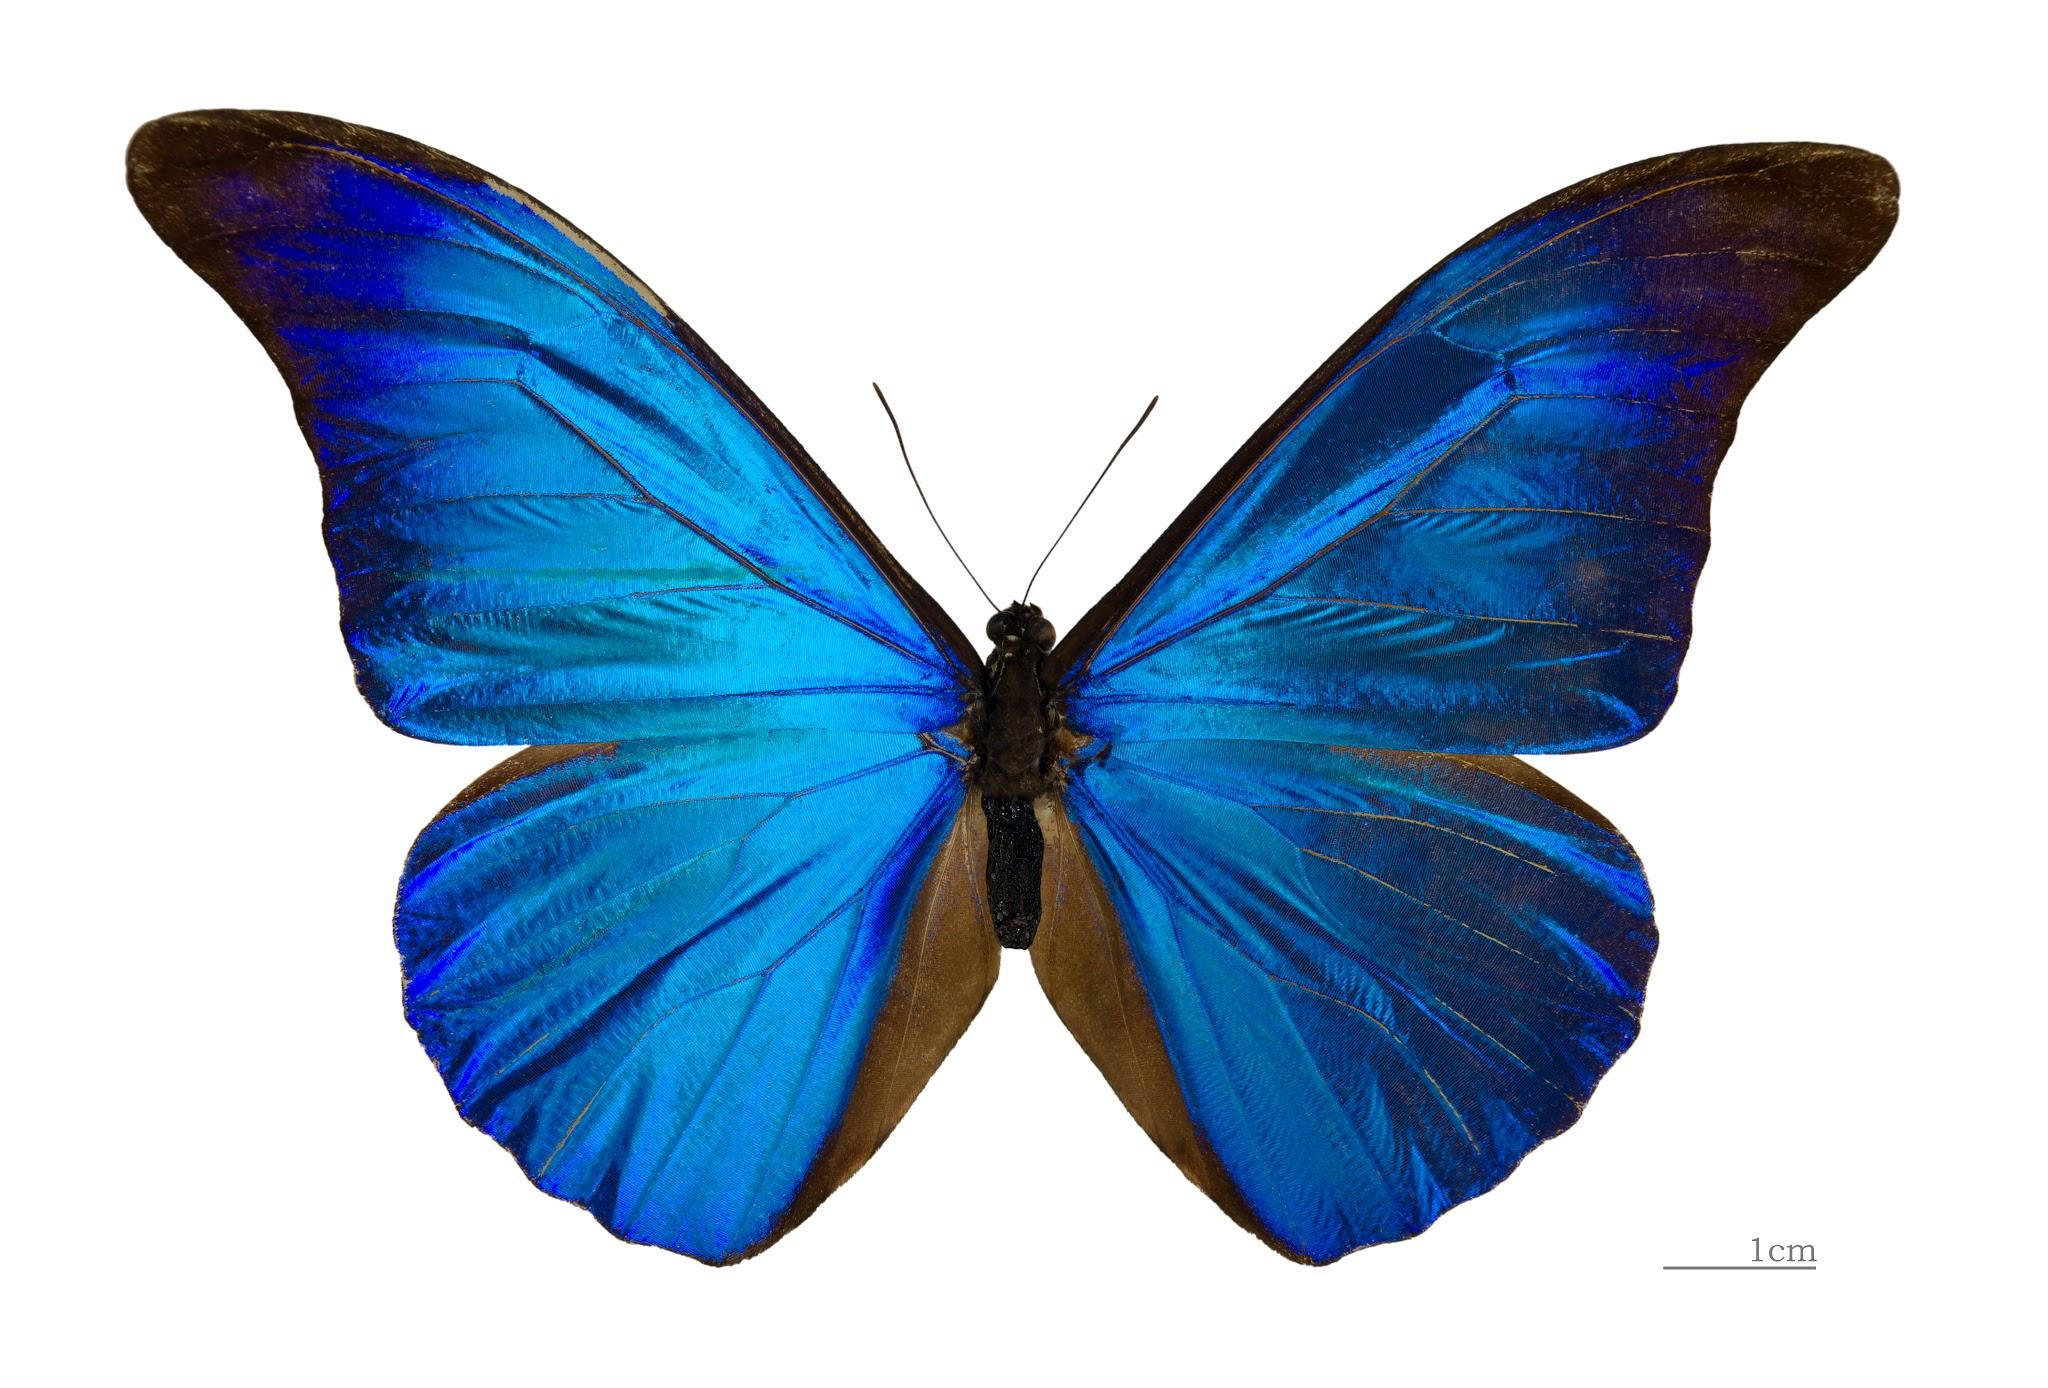
\includegraphics[width=\textwidth]{butterfly}
            [cry for help]
        \column{0.5\textwidth}
            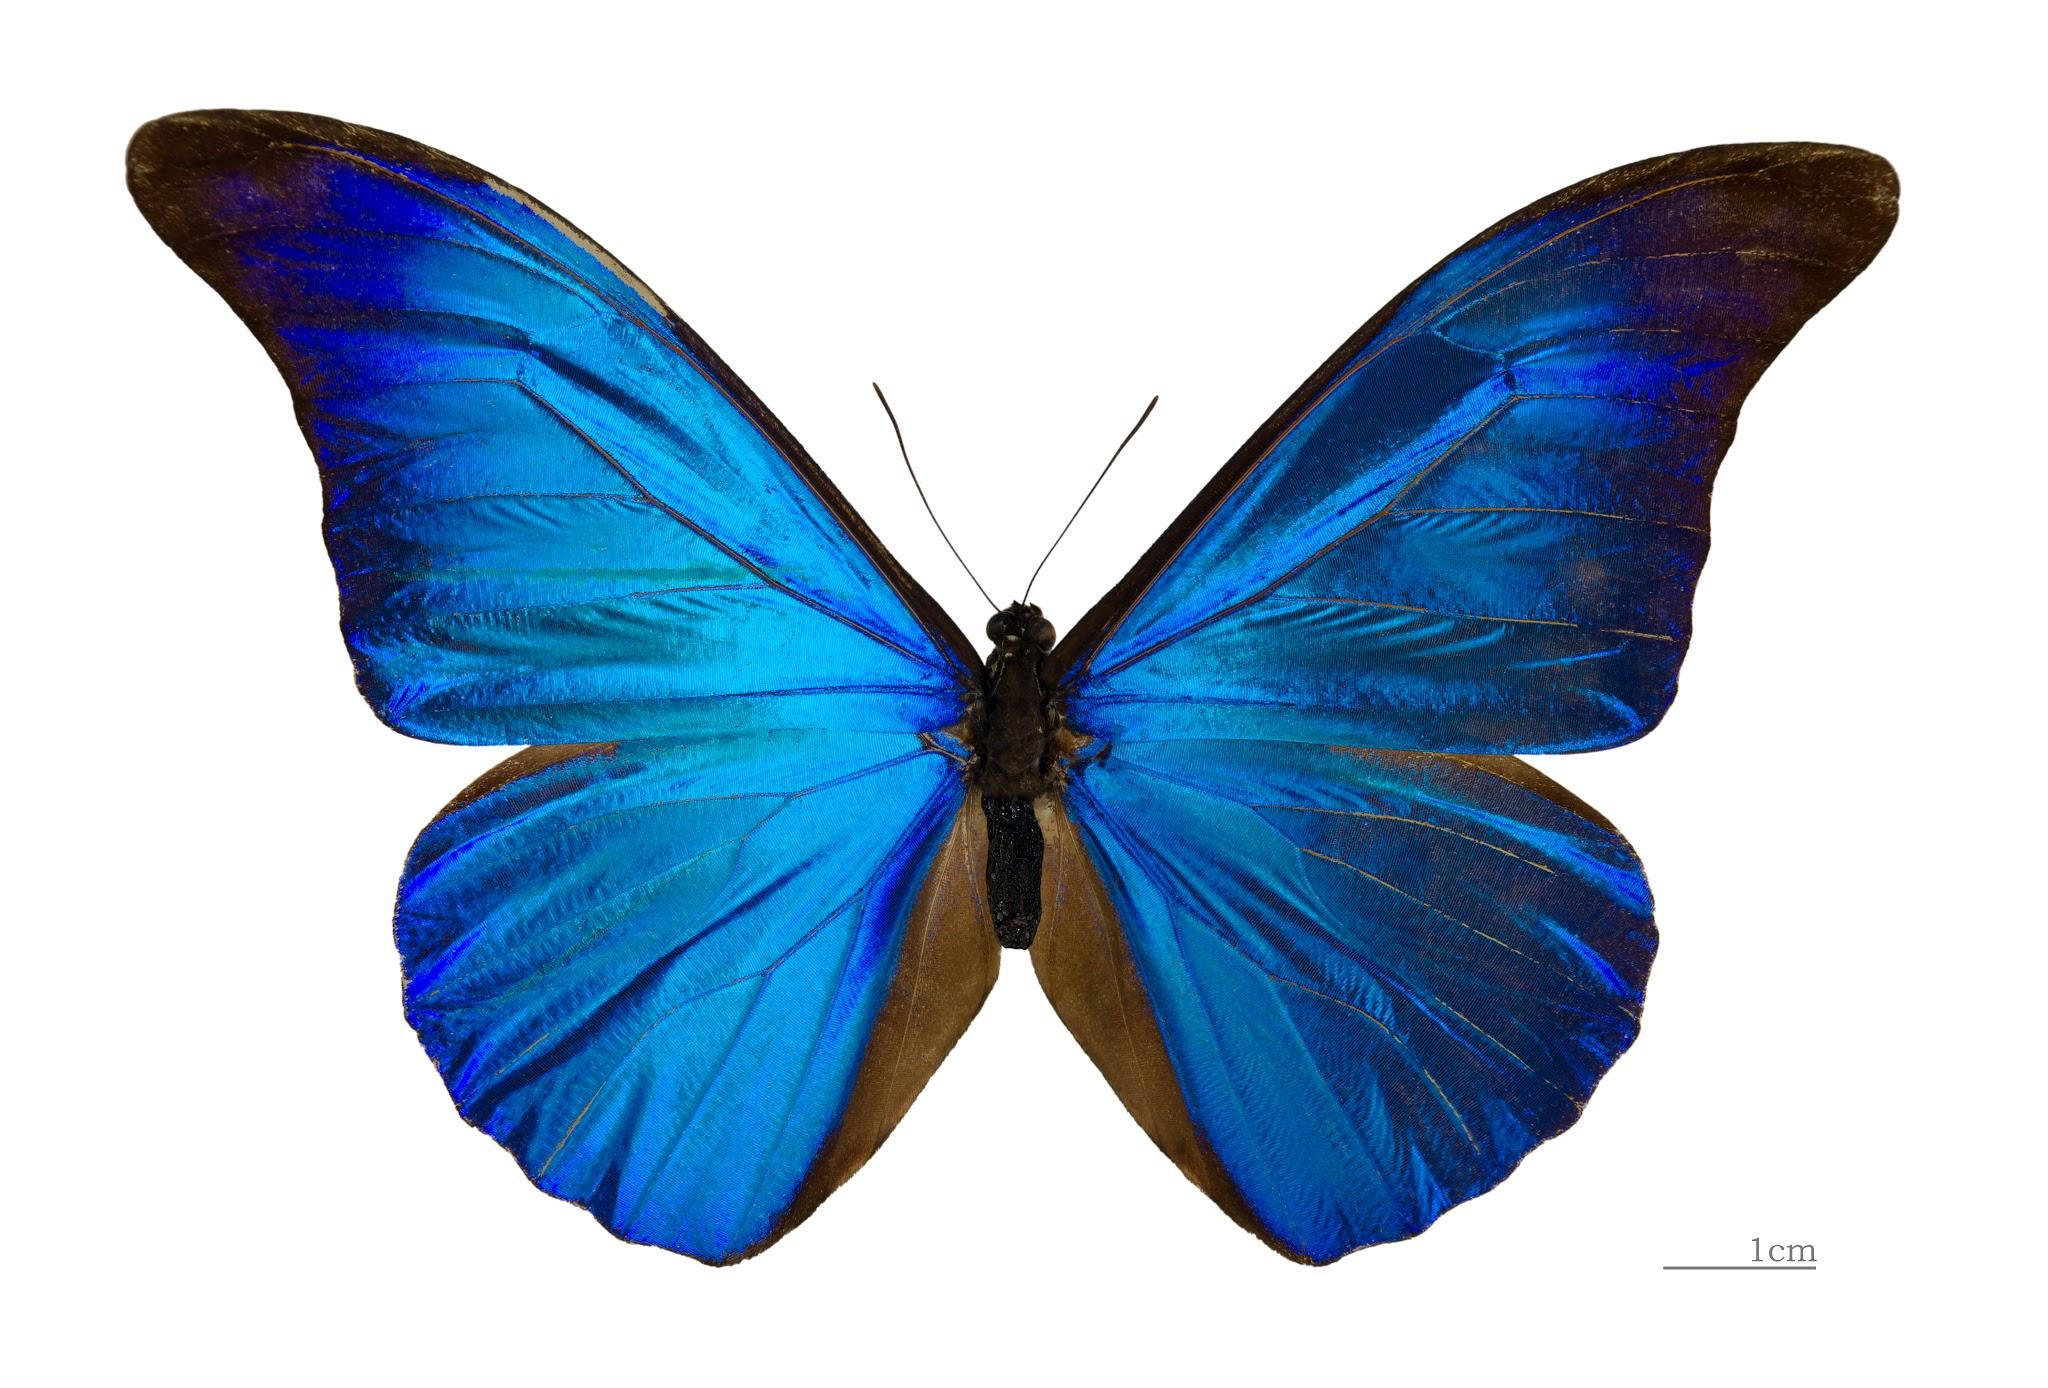
\includegraphics[width=\textwidth]{butterfly}
            \#Before: Recovery is a journey but I've come a long way
    \end{columns}    
\end{frame}

\begin{frame}{Public-Facing Policies}
    \begin{columns}
        \column{0.6\textwidth}
            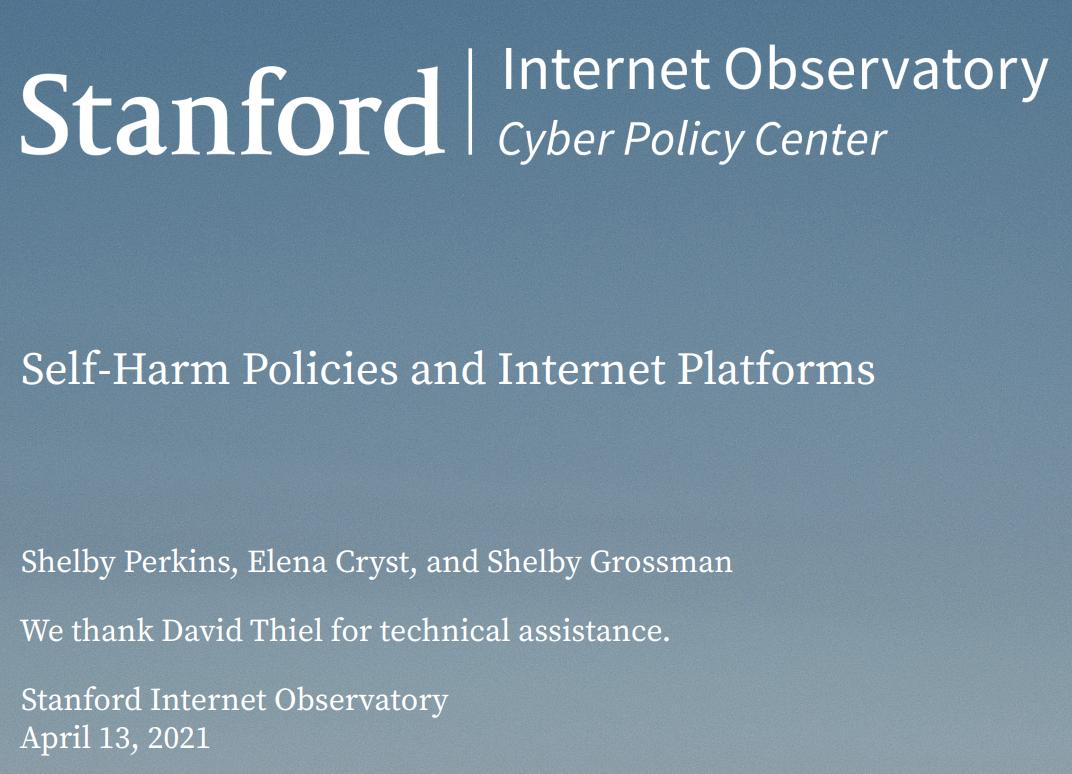
\includegraphics[width=\textwidth]{sio-self-harm-policies-report}
        \column{0.4\textwidth}
            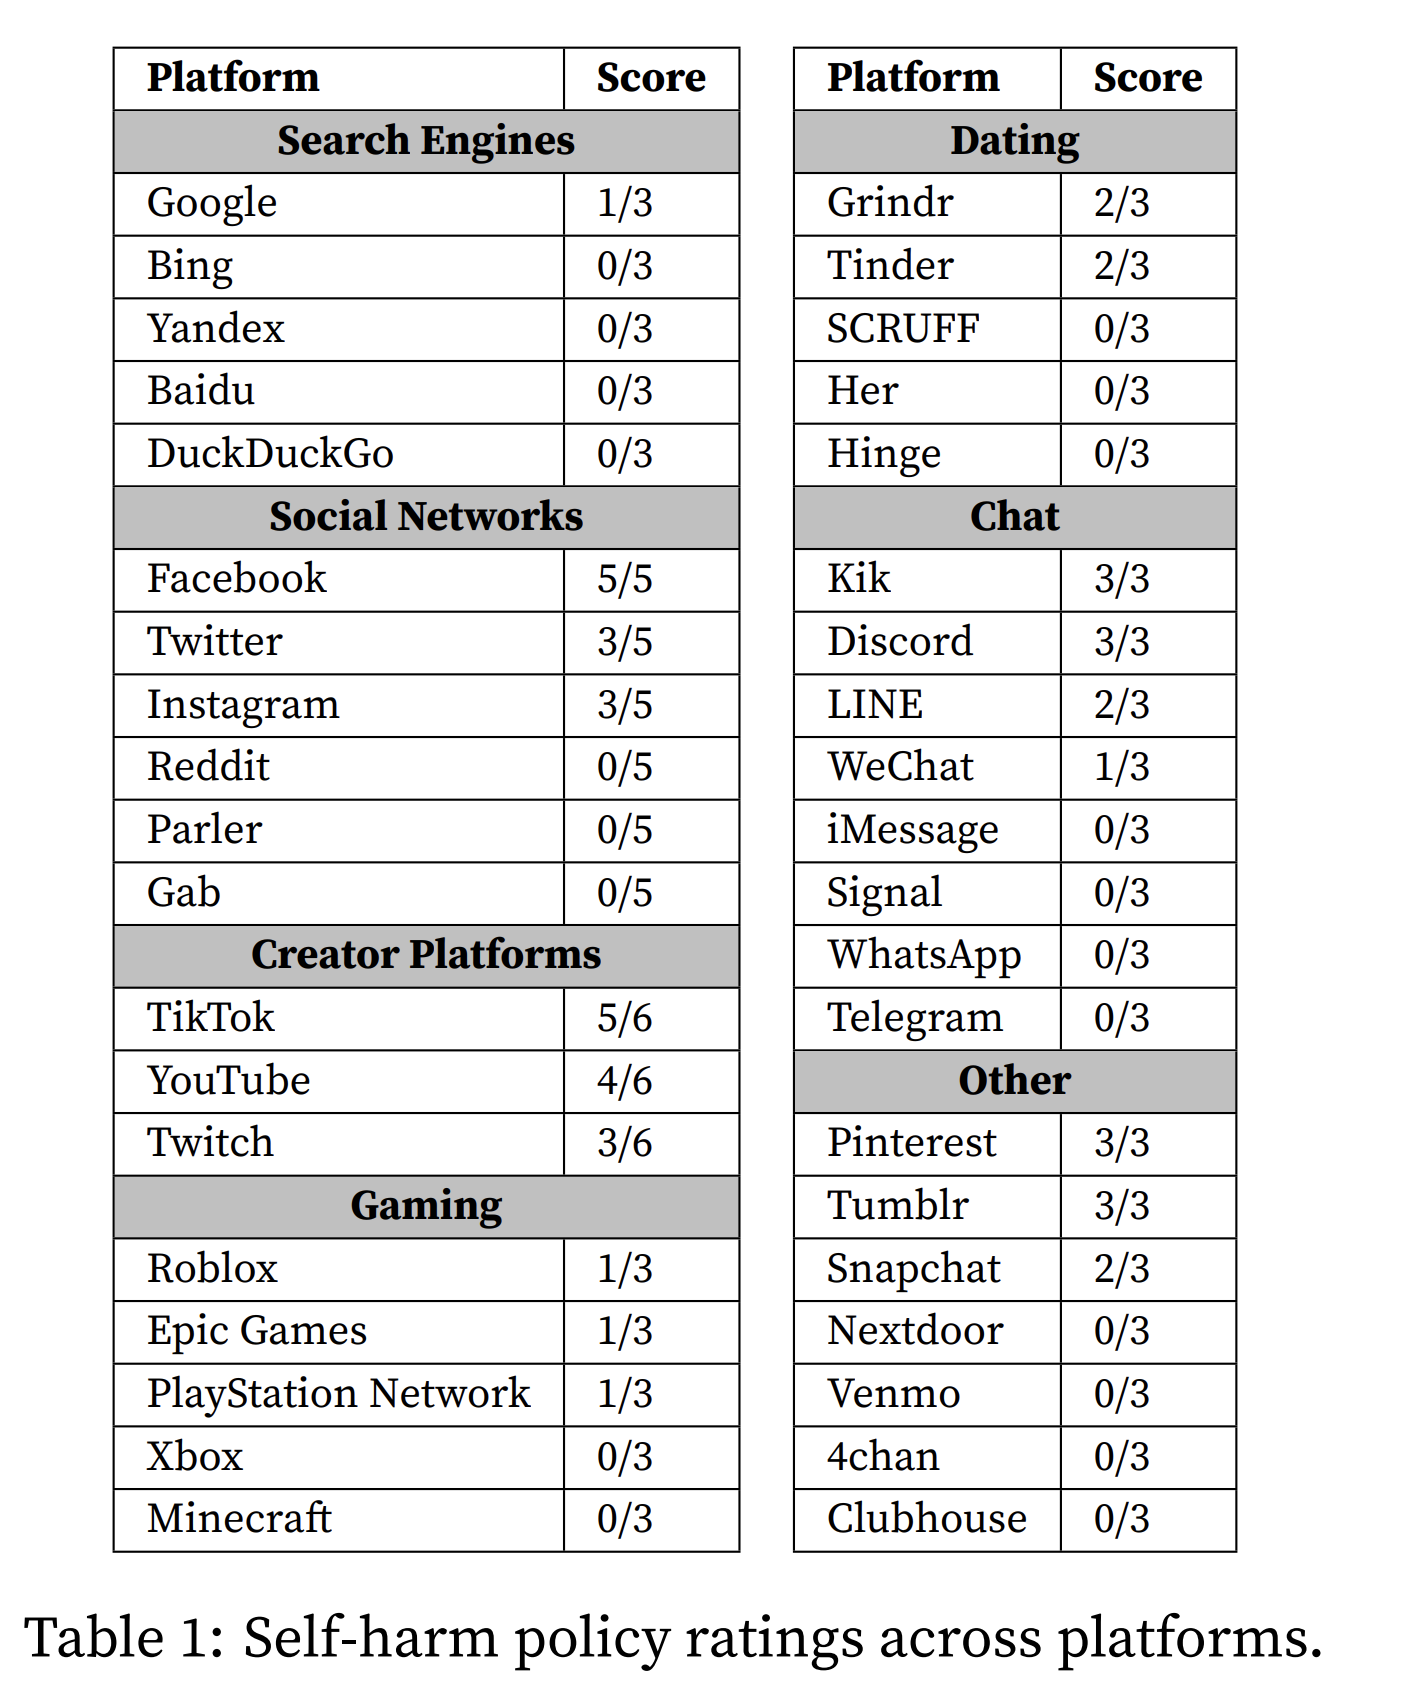
\includegraphics[width=\textwidth]{sio-self-harm-policies-table}
    \end{columns}
\end{frame}

\begin{frame}{Facebook v. YouTube}
    \begin{columns}
        \column{0.3\textwidth}
            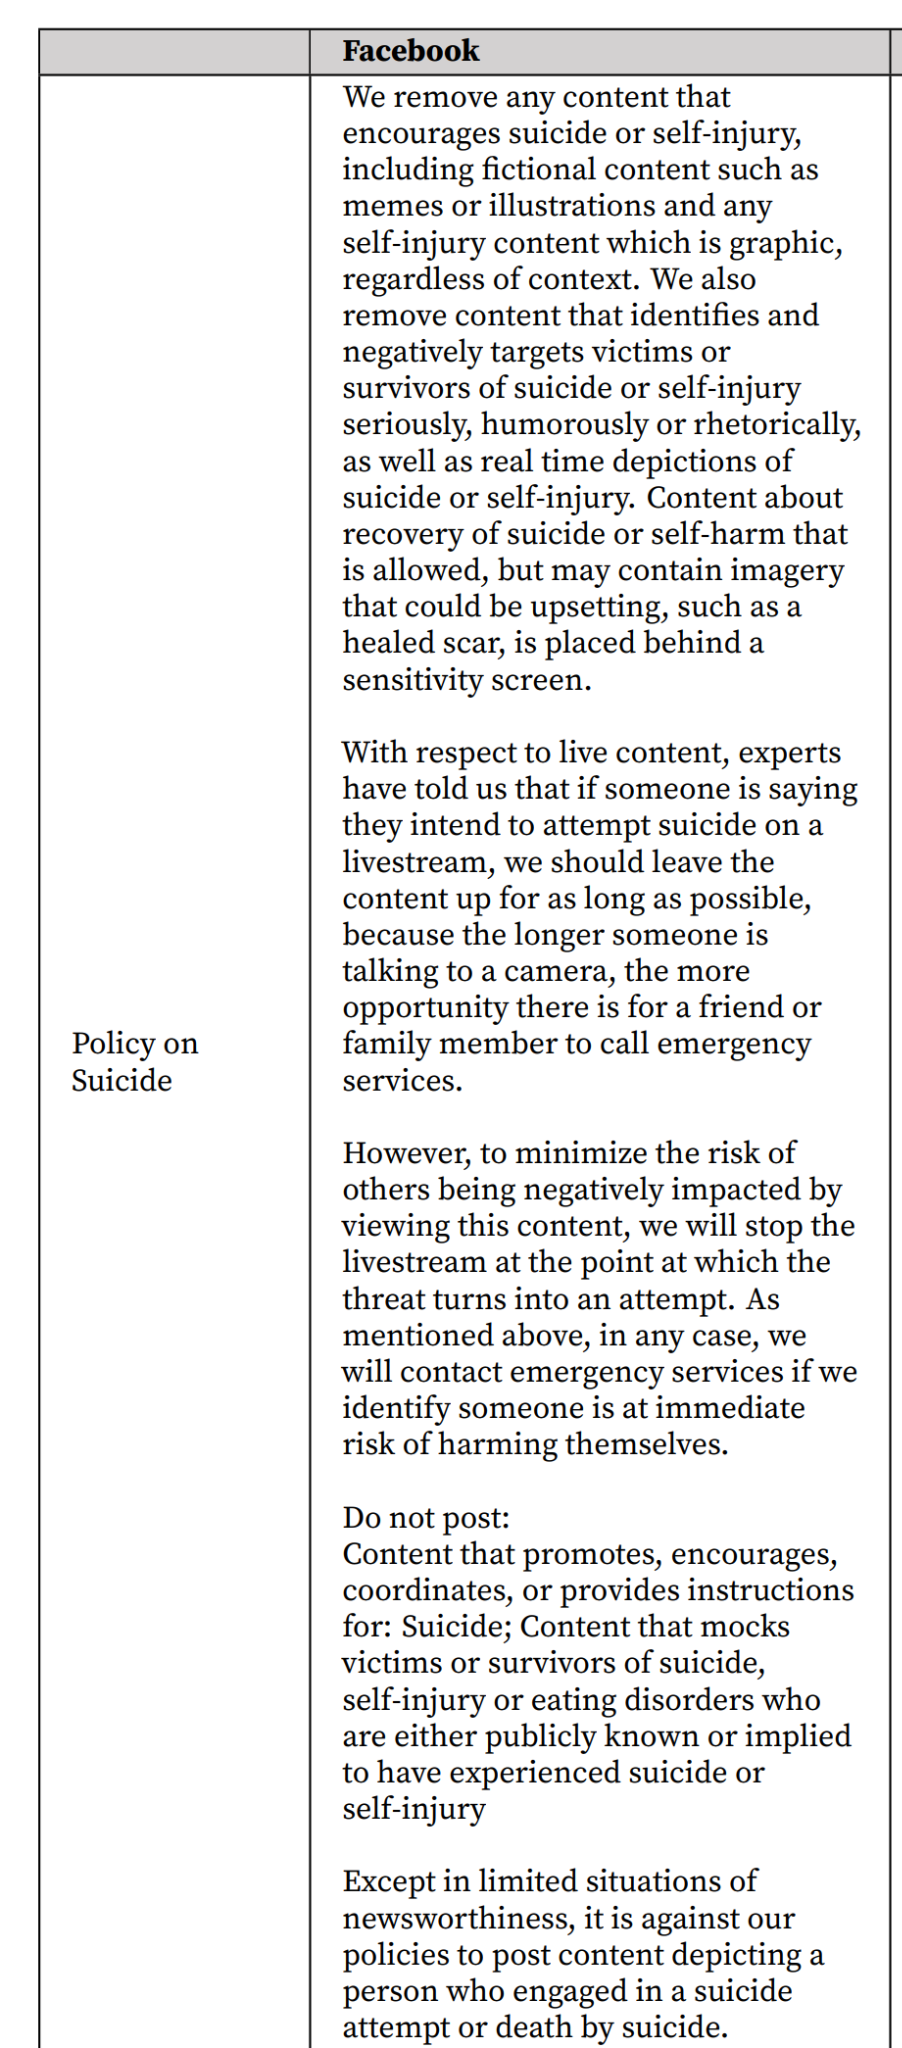
\includegraphics[width=\textwidth]{policy-on-suicide-facebook}
        \column{0.7\textwidth}
            \centering
            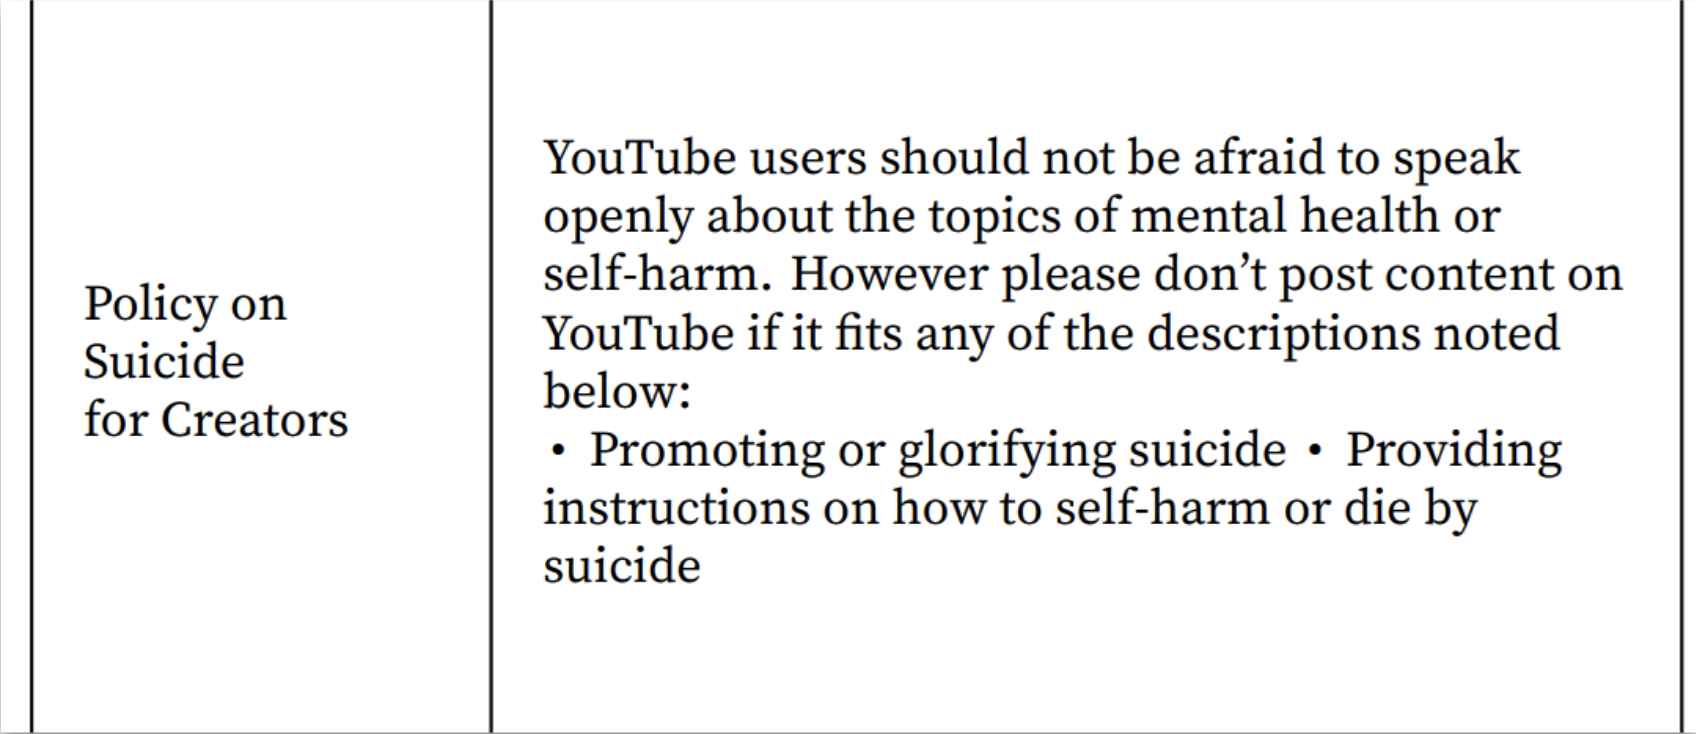
\includegraphics[width=0.75\textwidth]{policy-on-suicide-youtube}
            \tiny
            \url{https://stacks.stanford.edu/file/druid:tm443wf7913/20210408-Self-Harm-Policies-And-Internet-Platforms.pdf}
    \end{columns}
\end{frame}

\begin{frame}{When Do Suicide Prevention Hotlines Appear?}
    \begin{columns}
        \column{0.5\textwidth}
            \centering
            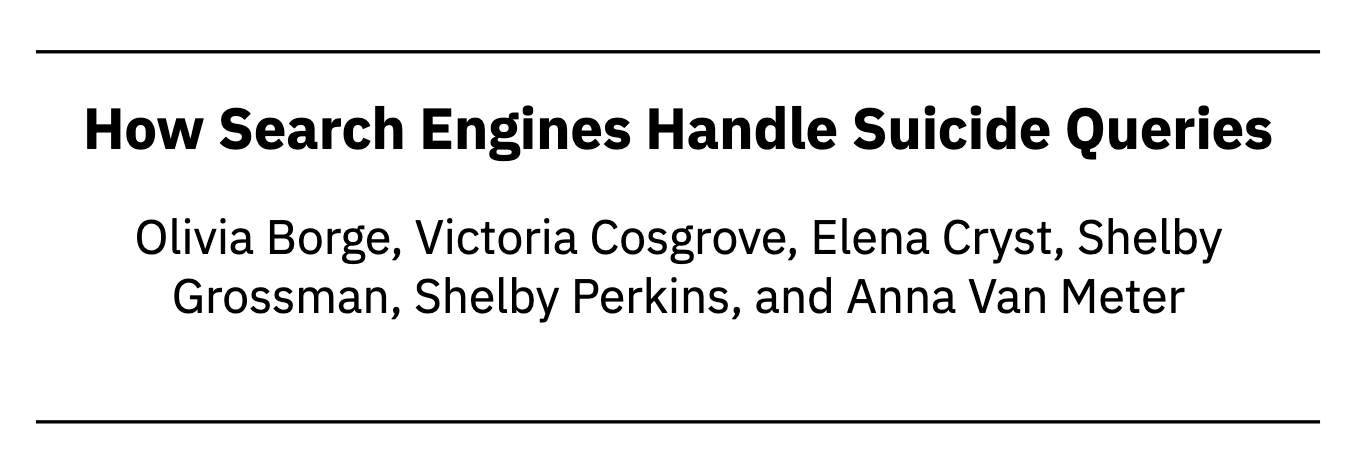
\includegraphics[width=0.9\textwidth]{hsehsq-title}
            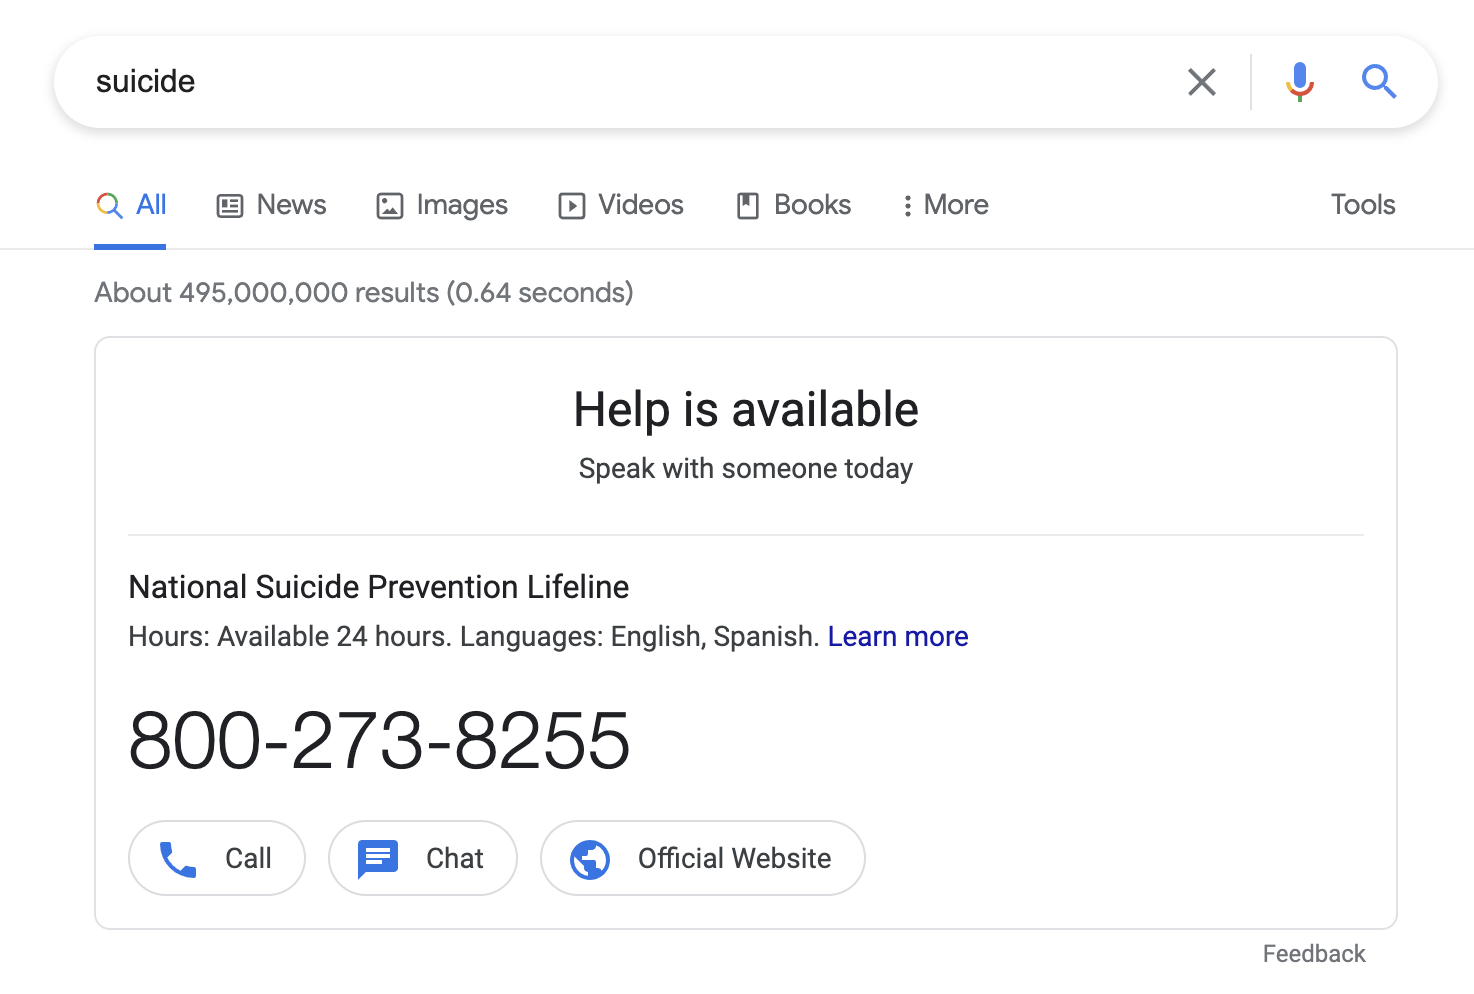
\includegraphics[width=\textwidth]{google-suicide-query-result}
            \tiny
            \url{https://tsjournal.org/index.php/jots/article/view/16/7}
        \column{0.5\textwidth}
            Study varies:
            \begin{itemize}
                \small
                \item Platform: Google, Bing, DuckDuckGo
                \item Query: General or specific/means-related
                \begin{itemize}
                    \footnotesize
                    \item People who go on to attempt to kill themselves frequently use specific queries
                \end{itemize}
                \item Language: English or Spanish
            \end{itemize}
    \end{columns}
\end{frame}

\begin{frame}{Google Provides Hotlines More Than Bing and DuckDuckGo}
    \centering
    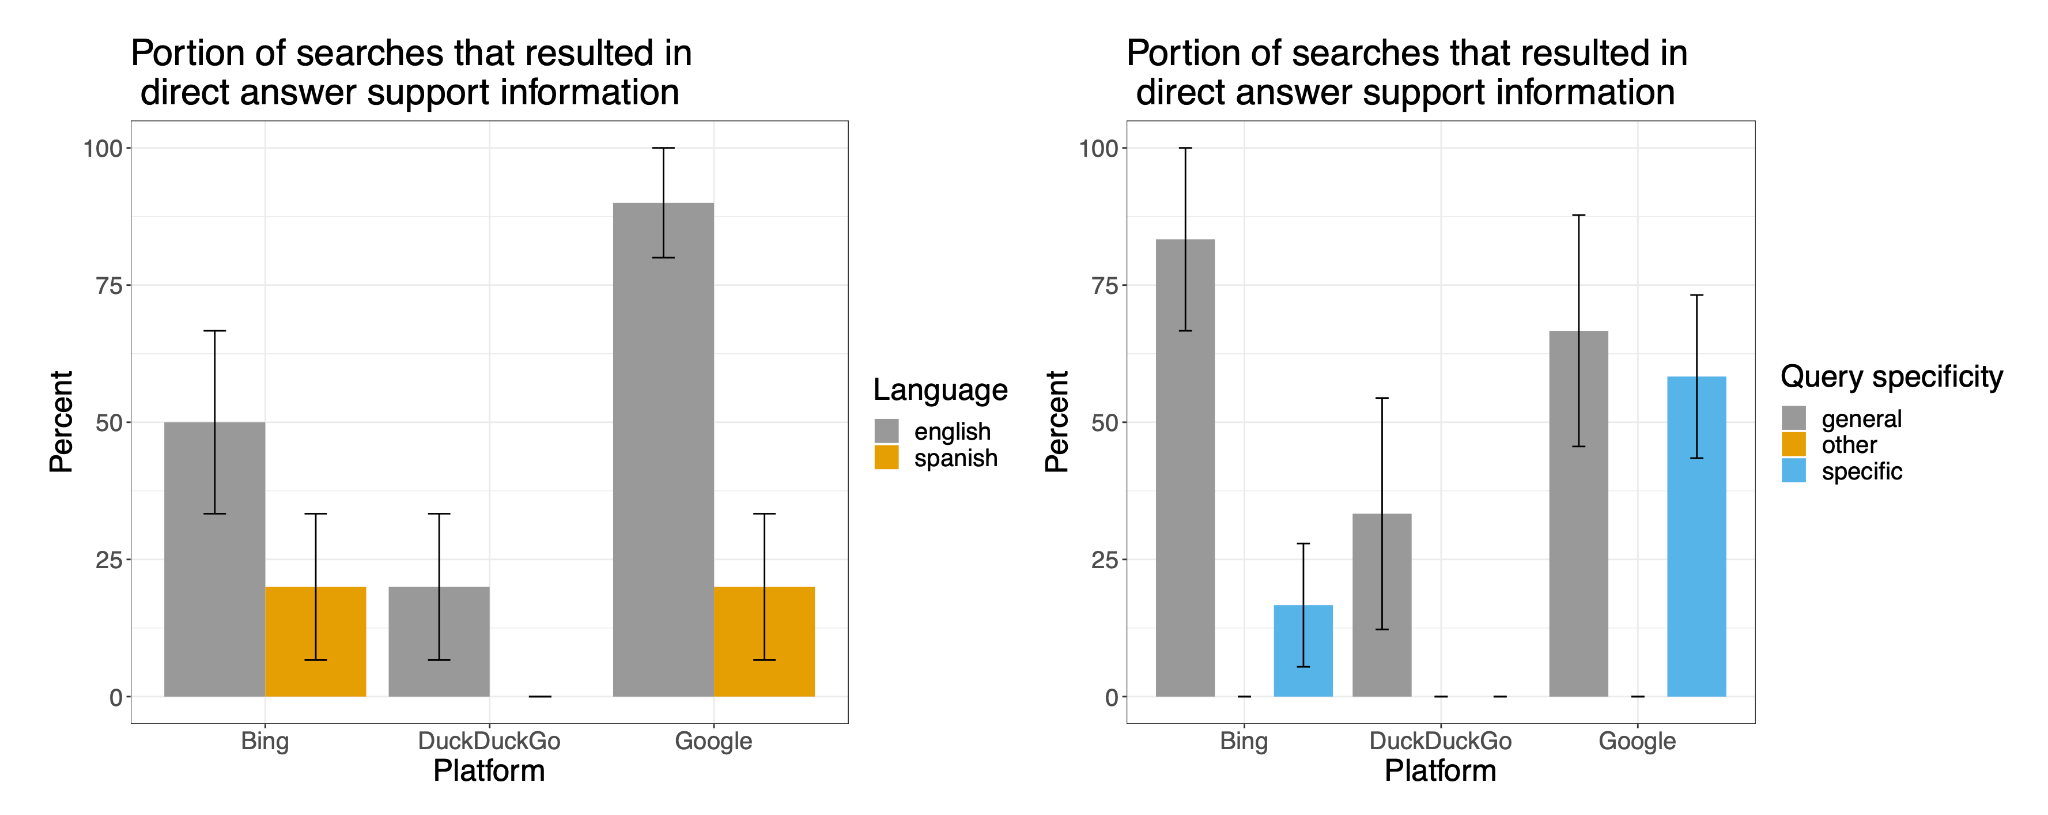
\includegraphics[width=\textwidth]{hsehsq-more-hotlines-provided}
    \tiny
    \url{https://tsjournal.org/index.php/jots/article/view/16/7}
\end{frame}

\begin{frame}{English Queries and Bing \& DuckDuckGo Most Harmful}
    \centering
    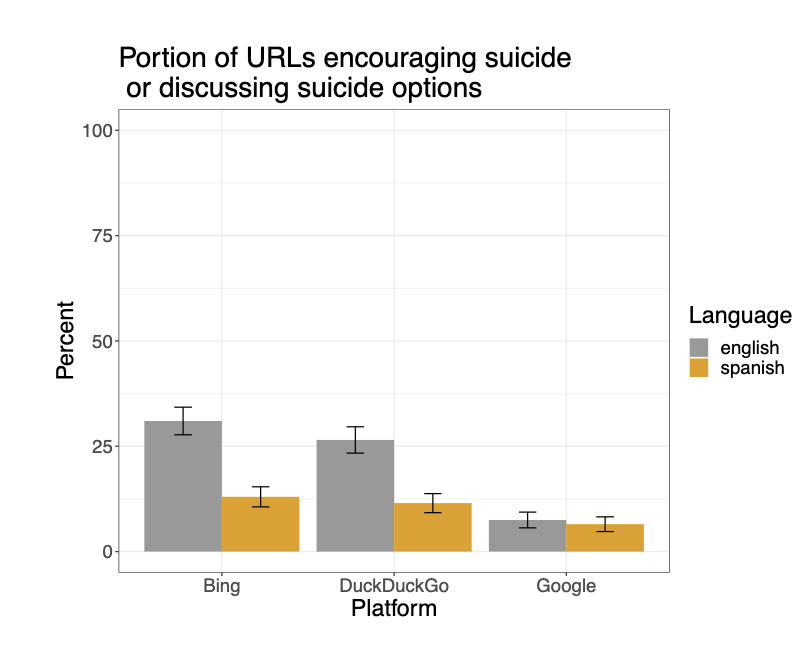
\includegraphics[height=0.75\textheight]{hsehsq-harmful-results}
    \tiny
    \url{https://tsjournal.org/index.php/jots/article/view/16/7}
\end{frame}

\begin{frame}{Specific, Means-Related Queries Surface Most Harmful URLs}
    \centering
    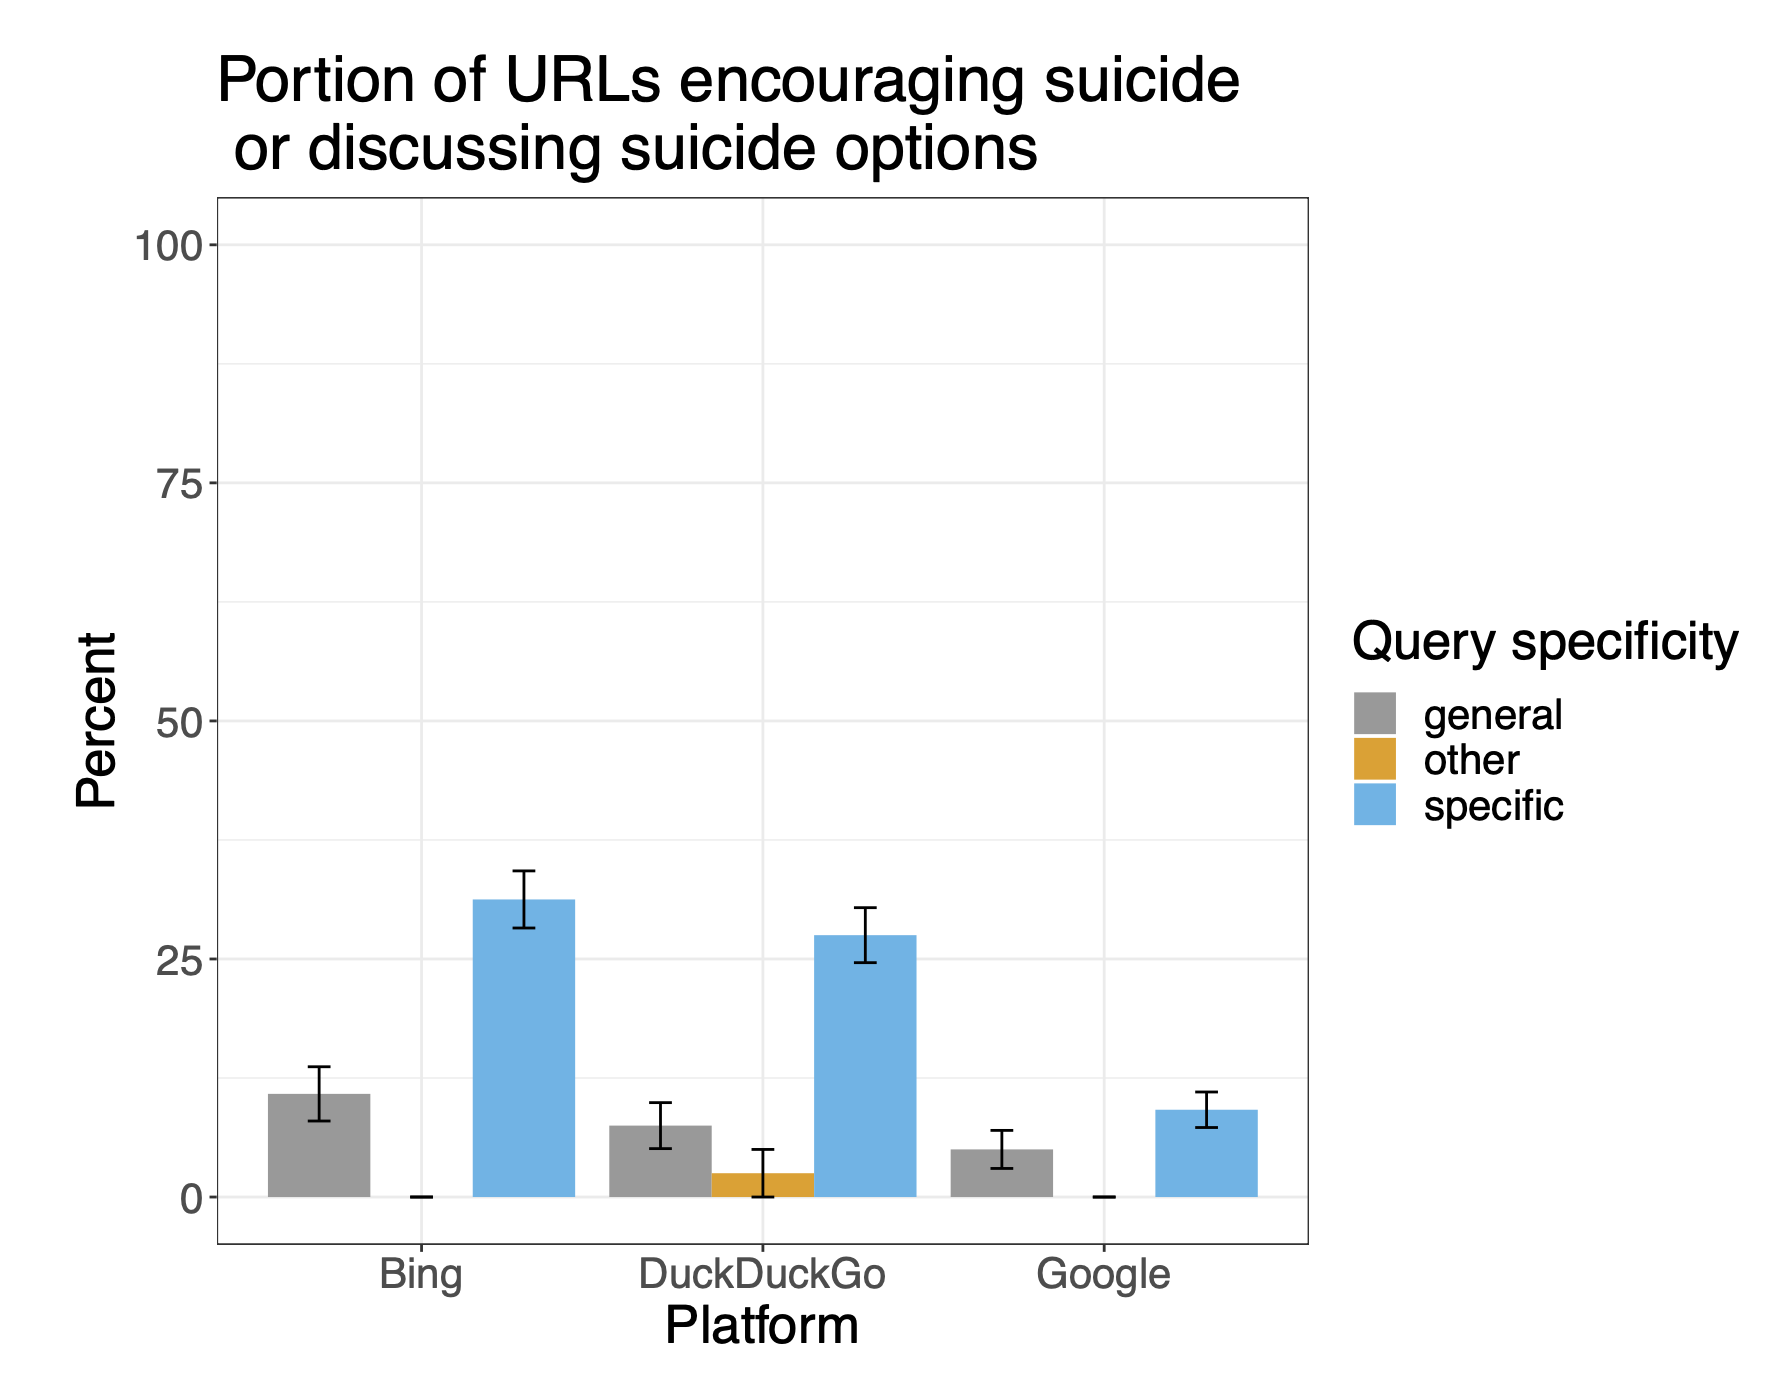
\includegraphics[height=0.75\textheight]{hsehsq-specific-most-harmful}
    \tiny
    \url{https://tsjournal.org/index.php/jots/article/view/16/7}
\end{frame}

\section{Product Design \& Past Interventions}

\begin{frame}{Product Design}
    \large
    It’s hard to create a perfect intervention.\\~\\
    This is an iterative process that is continually improving
\end{frame}

\begin{frame}{2010 - The First Intervention}
    \begin{columns}
        \column{0.45\textwidth}
            In 2010 at the suggestion of employees, Google launched a feature that displayed the National Suicide Prevention Lifeline as the top result for select search queries in the U.S.\\~\\
            It looked like this … 
        \column{0.55\textwidth}
            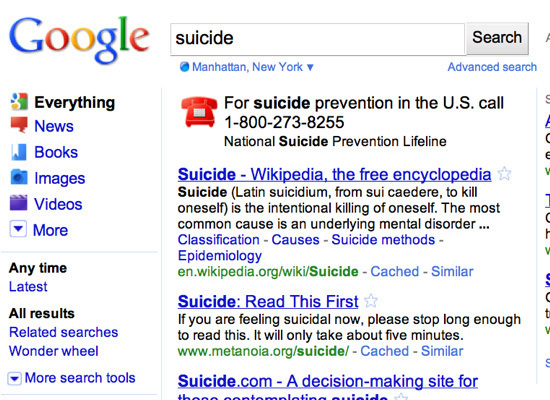
\includegraphics[width=\textwidth]{first-intervention}
    \end{columns}
\end{frame}

\begin{frame}{2012 - Restricting Discoverability}
    \begin{columns}
        \column{0.7\textwidth}
            \small
            In 2012, Instagram, Tumblr and Pinterest ban content glorifying eating disorders and implemented discoverability restrictions on hashtags and search terms\\
            \begin{itemize}
                \footnotesize
                \item Tumblr added PSAs to searches on tags including “anorexic,” “thinspo,” and “proana”
                \item Instagram announced that it would disable any account encouraging self harm behavior, add links to National Eating Disorder Awareness, and blocked searches on 17 hashtags including \#proanorexia and \#thighgap
                \item Pinterest banned search terms like “thinspiration” “thinterest,” removed content, and added PSAs
            \end{itemize}
        \column{0.3\textwidth}
            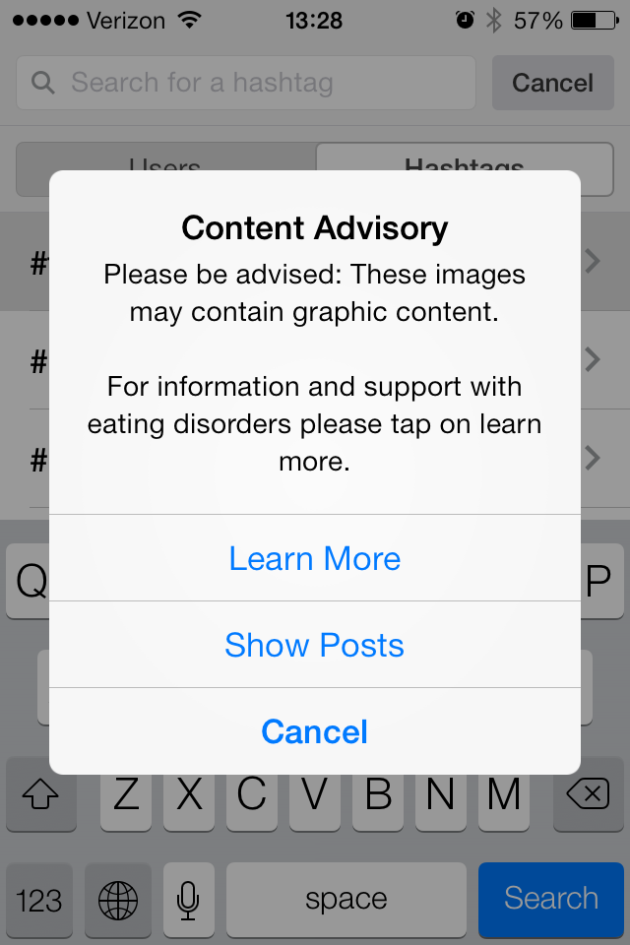
\includegraphics[width=\textwidth]{restricted-discoverability}
    \end{columns}
\end{frame}

\begin{frame}{2012 - Restricting Discoverability}
    \textit{These changes were mostly ineffective}\\~\\
    \begin{tabular}{|c|c|c|}%TODO fix table
         \hline
         \textbf{Root Tag} & \textbf{\#Var.} & \textbf{Lexical Variants}\\
         \hline
         anorexia & 99 & anorexic, anorexie, anoressia, anorexi, anorexia, anorexique, anorexica, anorectic, anorexia, anoretic\\
         \hline
         bulimia & 49 & bulimic, bulima, bulimie, bulimi, bulimia, bulimica, bulimc, bulimiaaa, bulimic, bulimist\\
         \hline
         thighgap & 107 & thighgaps, thygap, thighgapp, thigh_gap, thightgap, thyghgap, thighgappp, thegap, thigap, thighgapss\\
         \hline
         thinspiration & 101 & thynspiration, thinsperation, thinspire, thynsporation, thinsporation, thinspiring, thinspirationn, thinspirational, thinsparation, thynsperation\\
         \hline
    \end{tabular}
    \tiny
    \textit{Stevie Chancellor, Jessica Annette Pater, Trustin Clear, Eric Gilbert, and Munmun De Choudhury. 2016. “\#thyghgapp: Instagram Content Moderation and Lexical Variation in Pro-Eating Disorder Communities.” In Proceedings of the 19th ACM Conference on Computer-Supported Cooperative Work \& Social Computing (CSCW '16). Association for Computing Machinery, New York, NY, USA, 1201–1213.}
\end{frame}

\begin{frame}{2016 - Anonmyous Reporting on Instagram}
    \begin{columns}
        \column{0.6\textwidth}
            \large
            Updated reporting flows allow users to anonymously report friends or contacts’ posts
        \column{0.4\textwidth}
            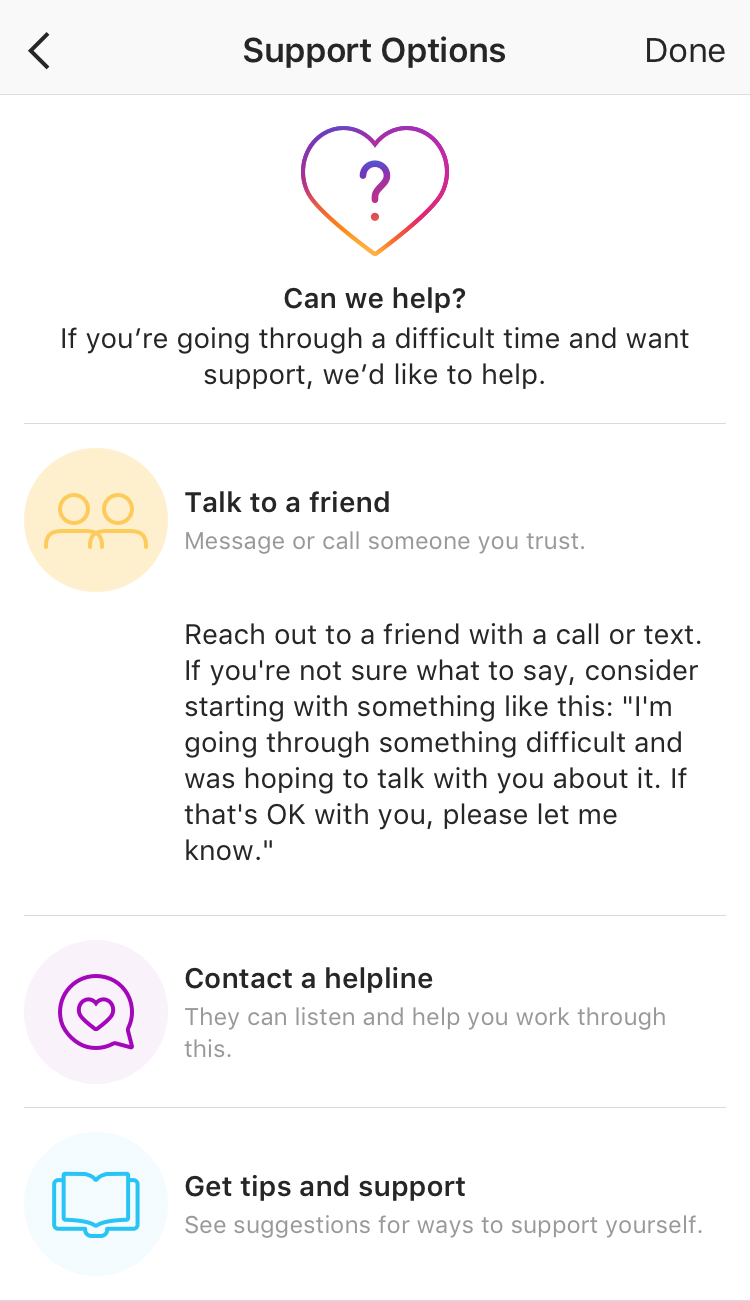
\includegraphics[width=\textwidth]{anonymous-reporting-instagram}
    \end{columns}
\end{frame}

\begin{frame}{Reporting Flow for Facebook Live Today}
    \begin{columns}
        \column{0.25\textwidth}
            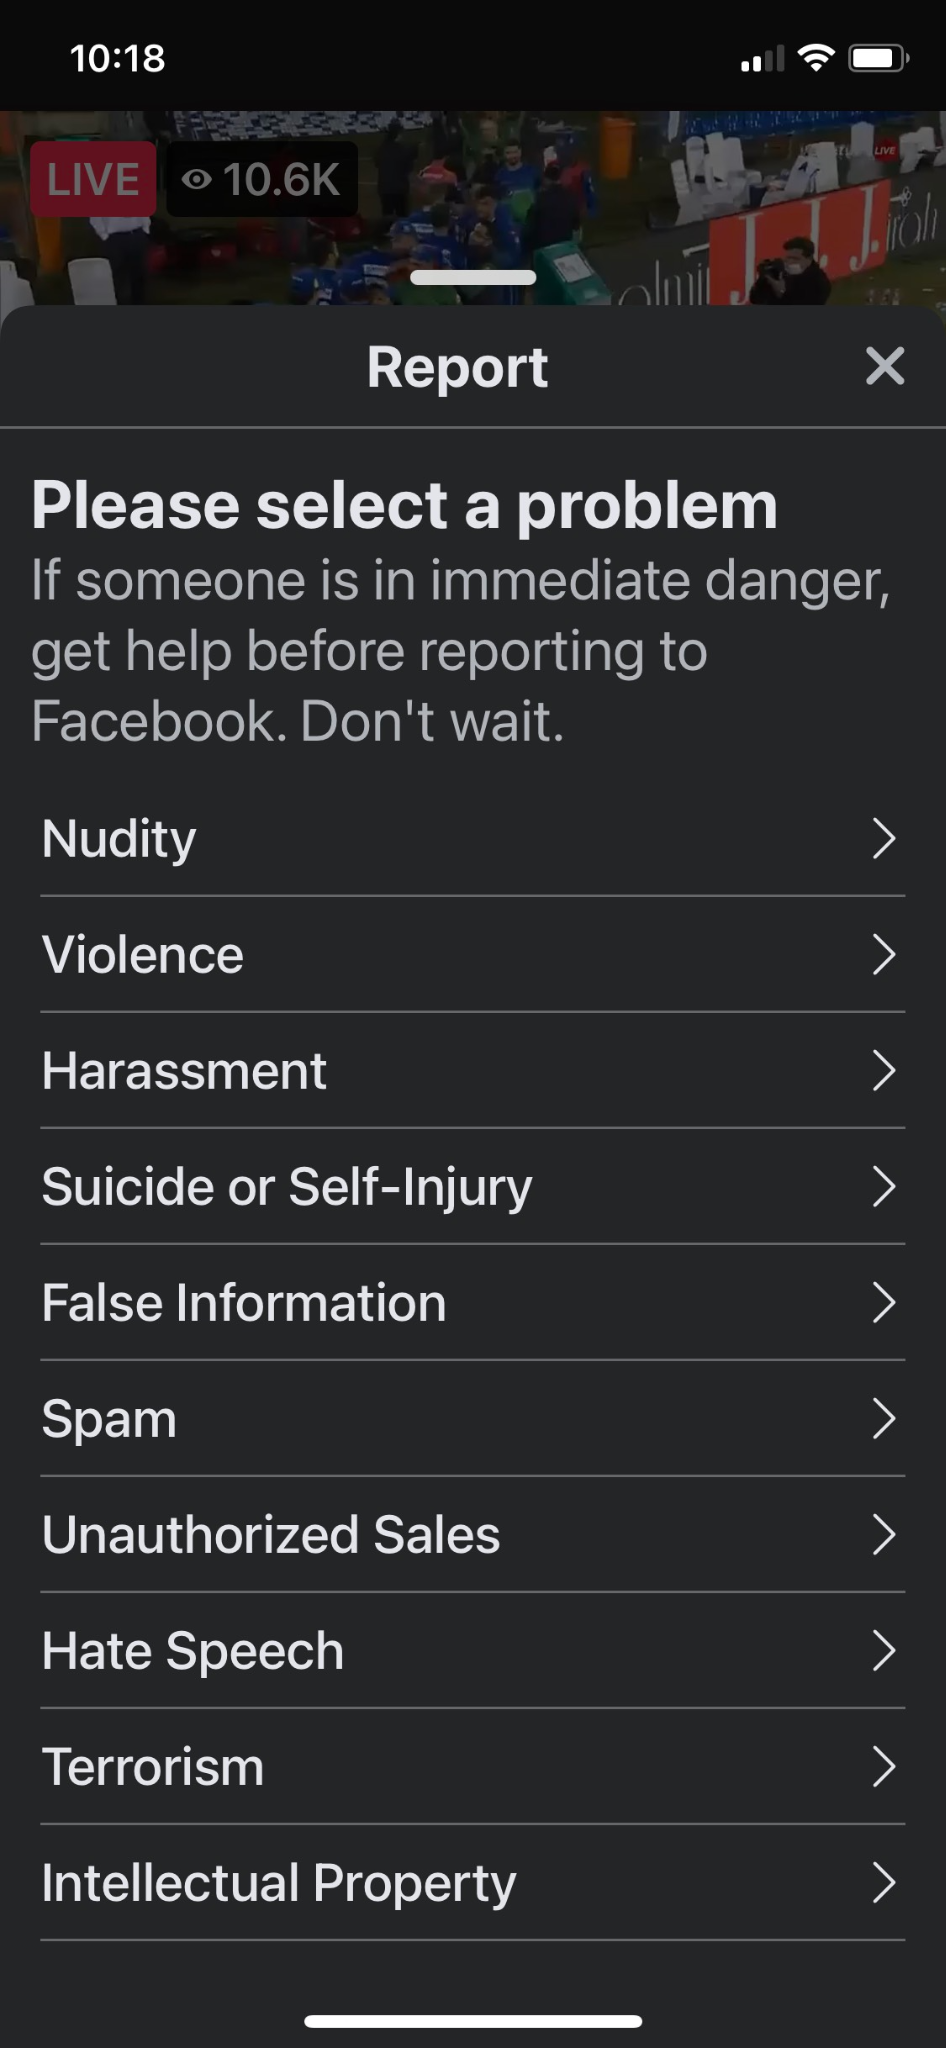
\includegraphics[width=\textwidth]{facebook-live-current-reporting-flow-1}
        \column{0.25\textwidth}
            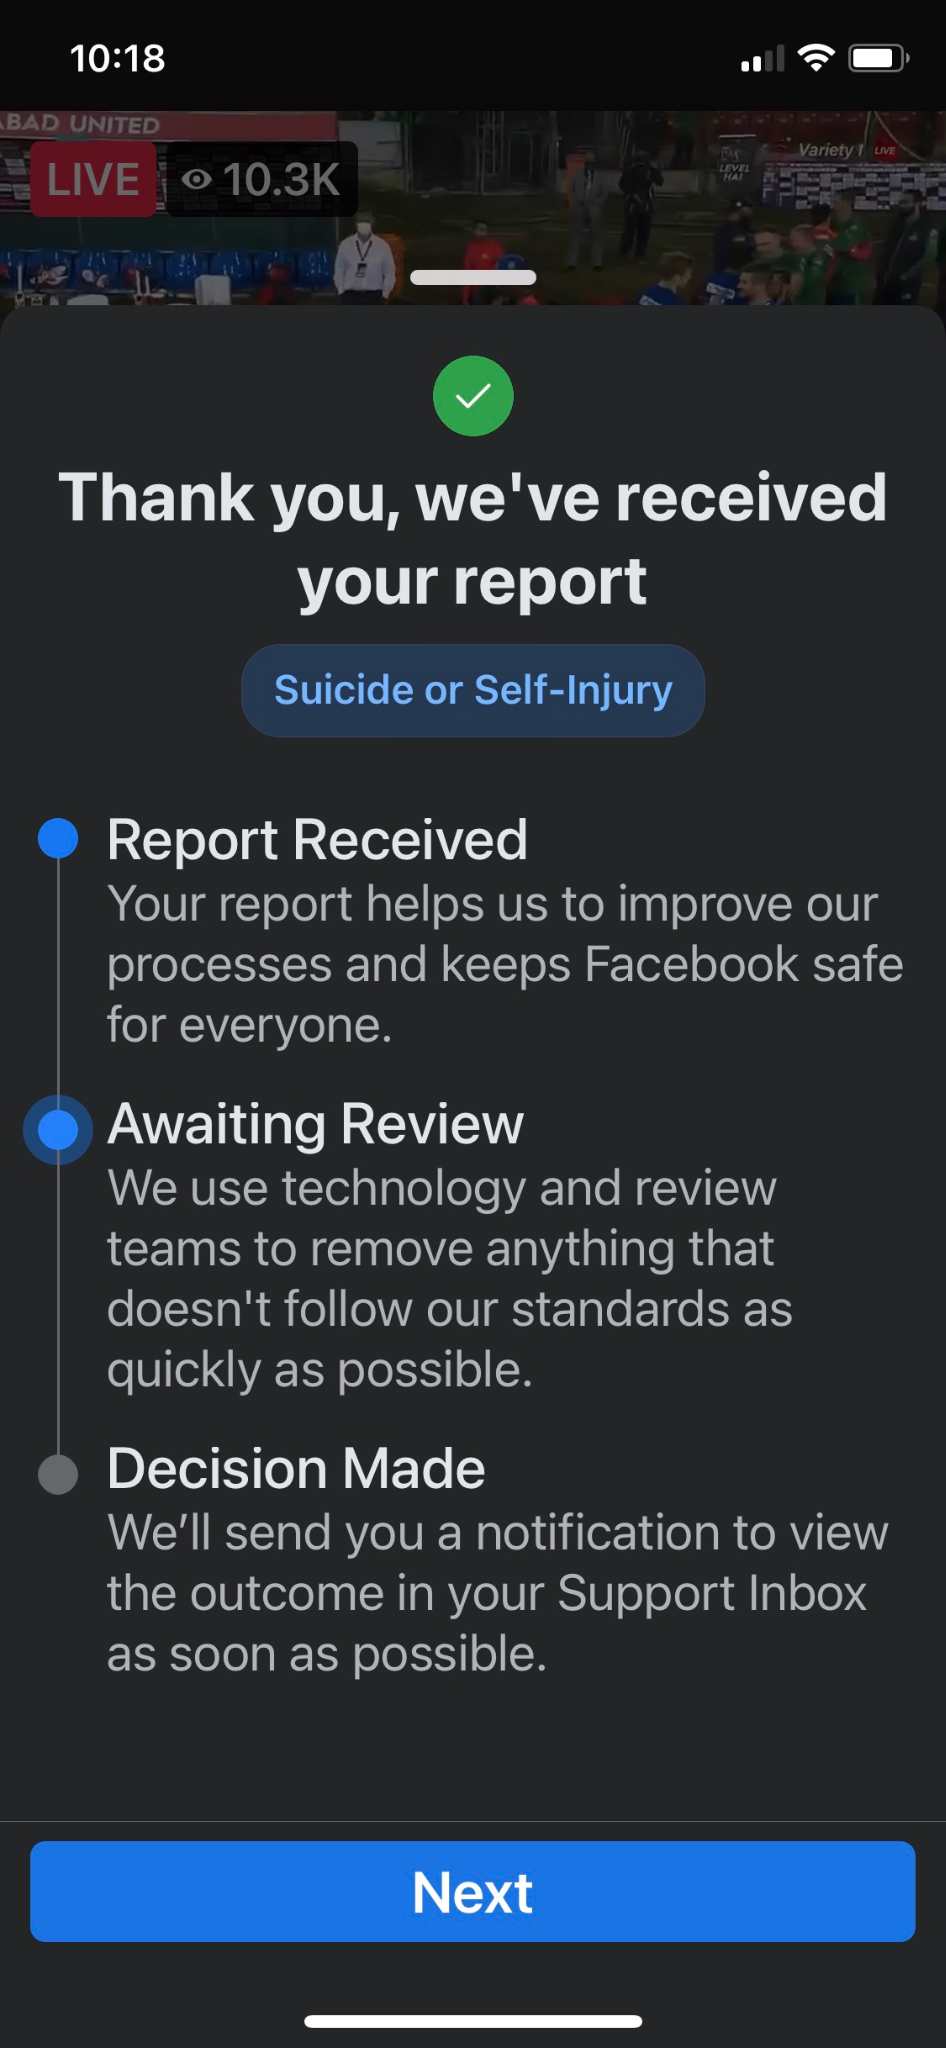
\includegraphics[width=\textwidth]{facebook-live-current-reporting-flow-2}
        \column{0.25\textwidth}
            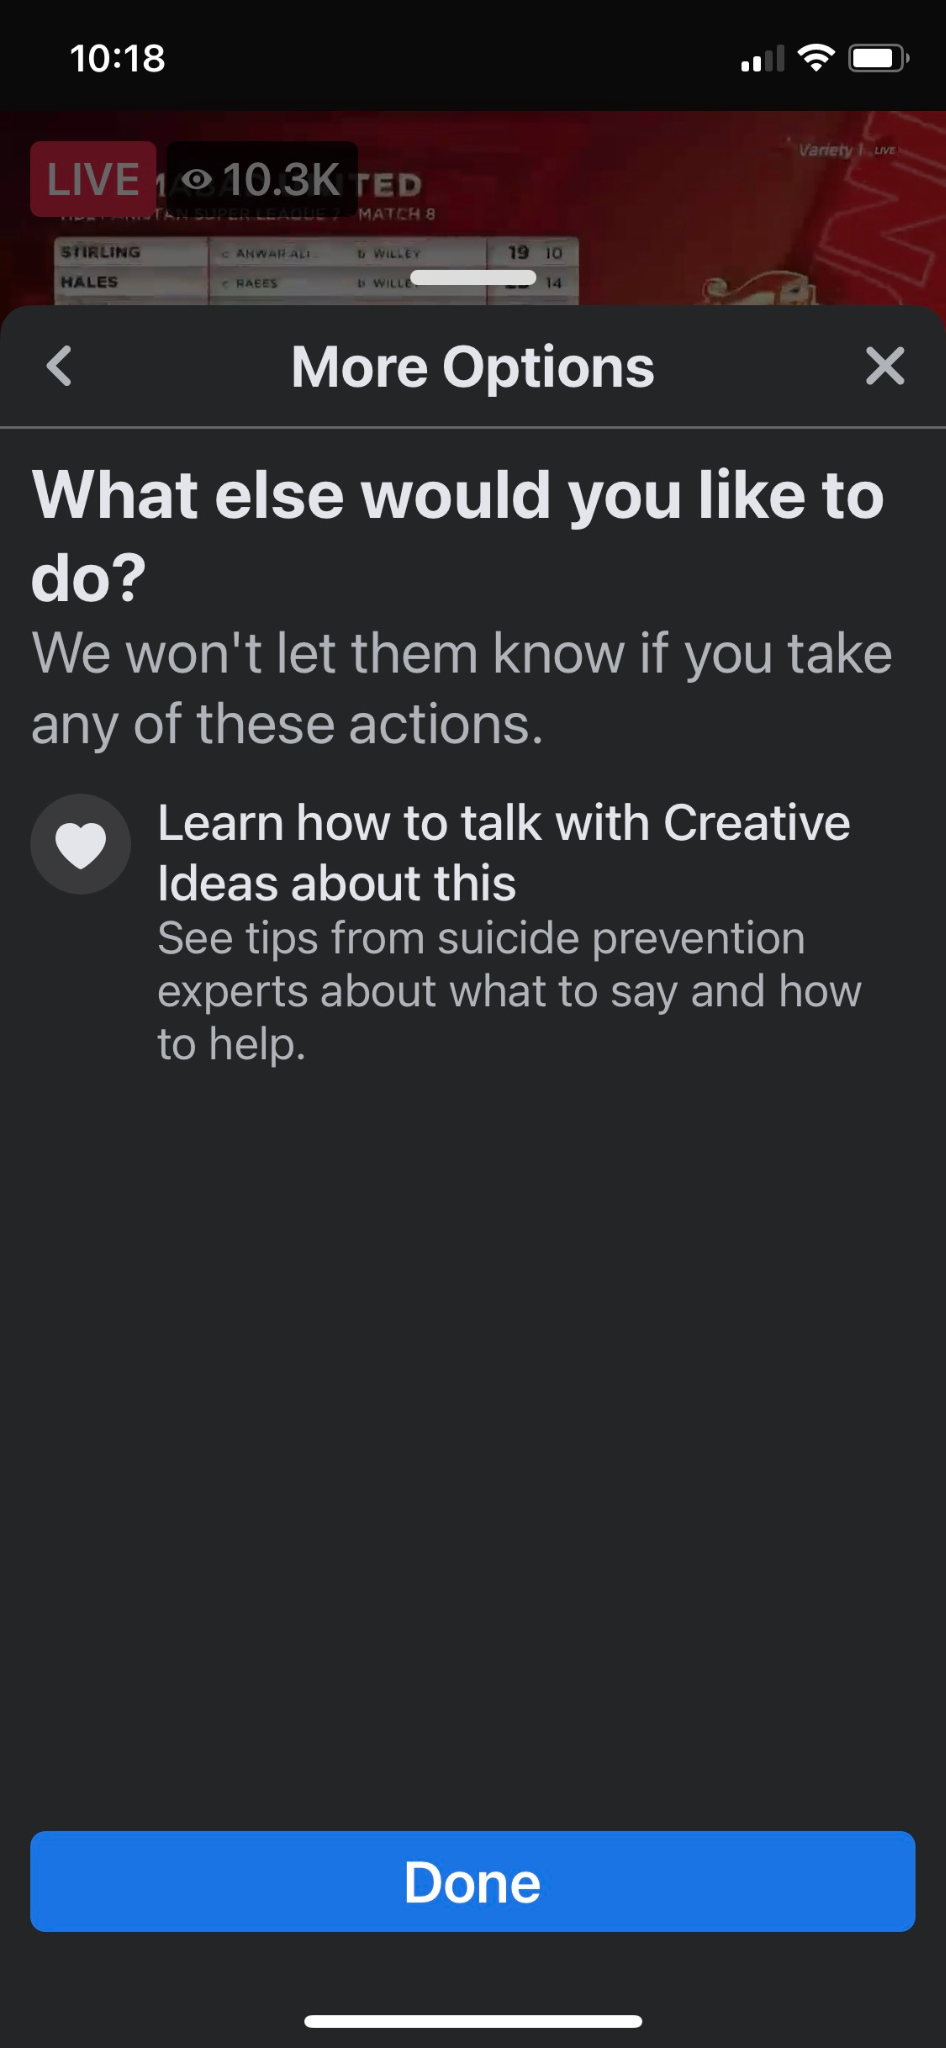
\includegraphics[width=\textwidth]{facebook-live-current-reporting-flow-3}
        \column{0.25\textwidth}
            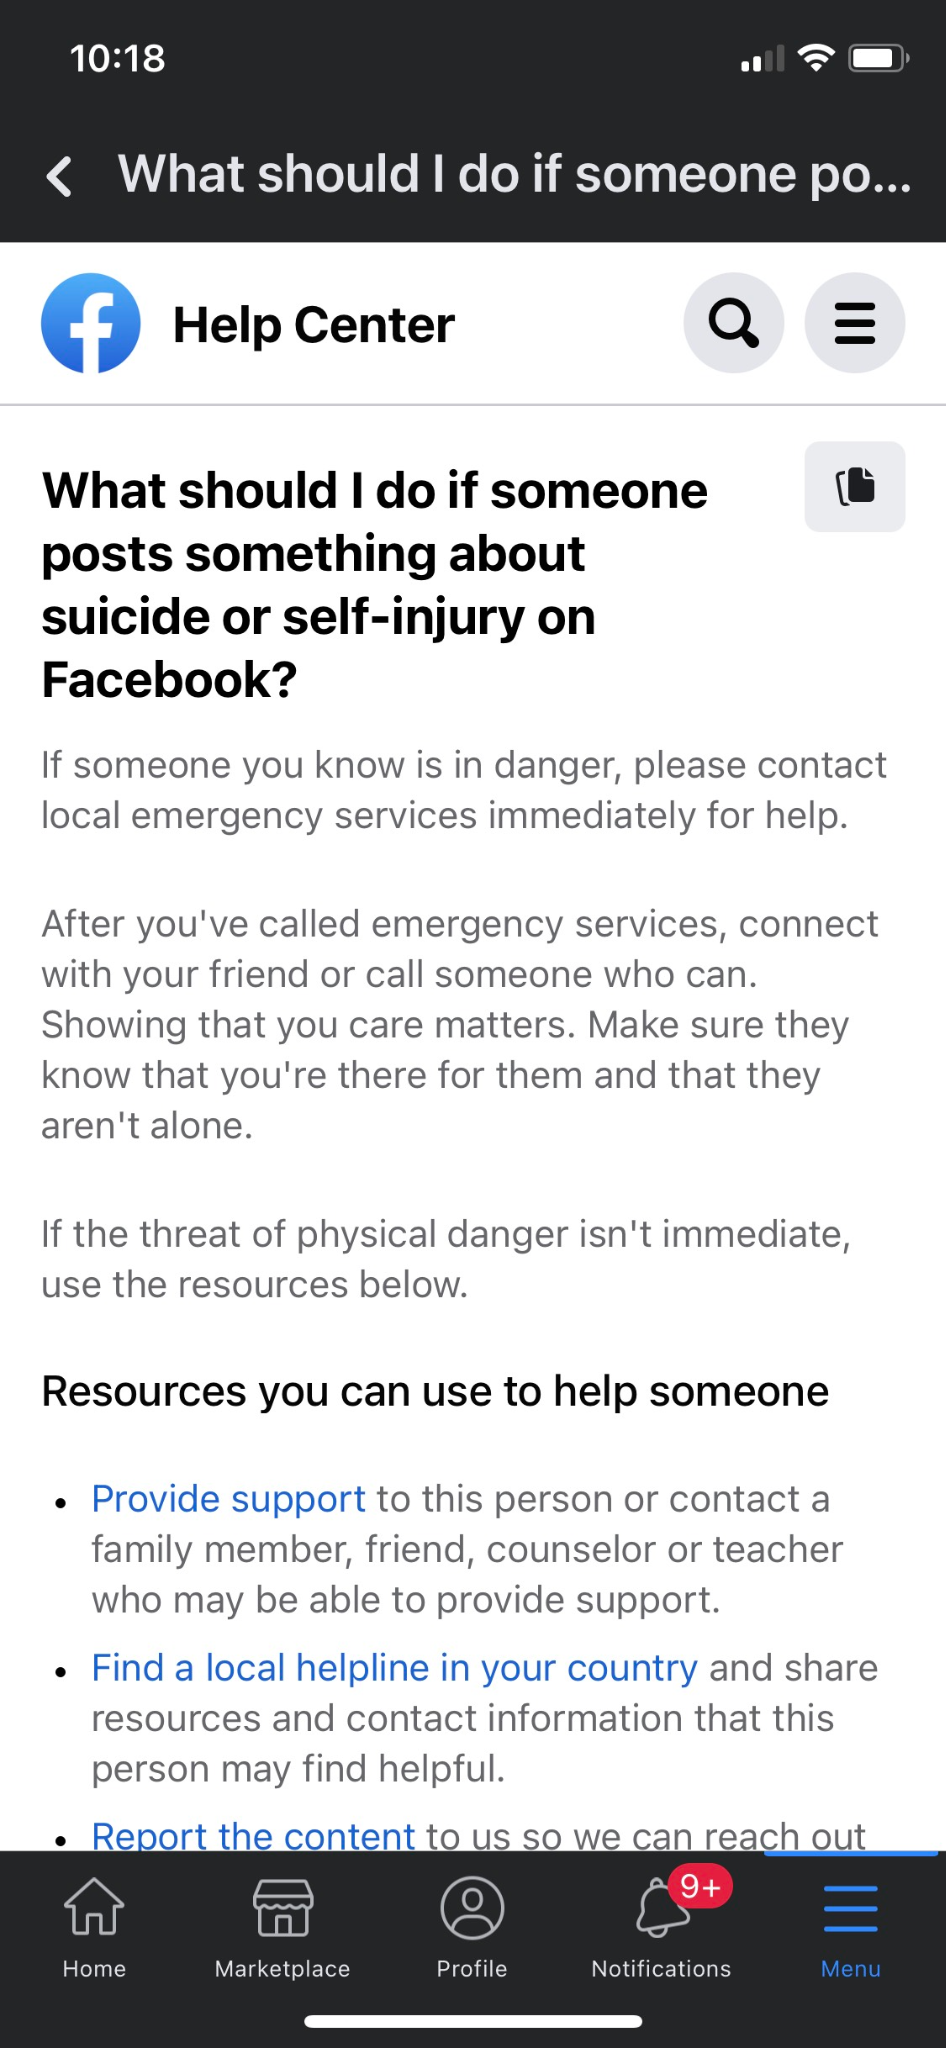
\includegraphics[width=\textwidth]{facebook-live-current-reporting-flow-4}
    \end{columns}
\end{frame}

\begin{frame}{2017 - Facebook Adds Screening and Alert Algorithms}
    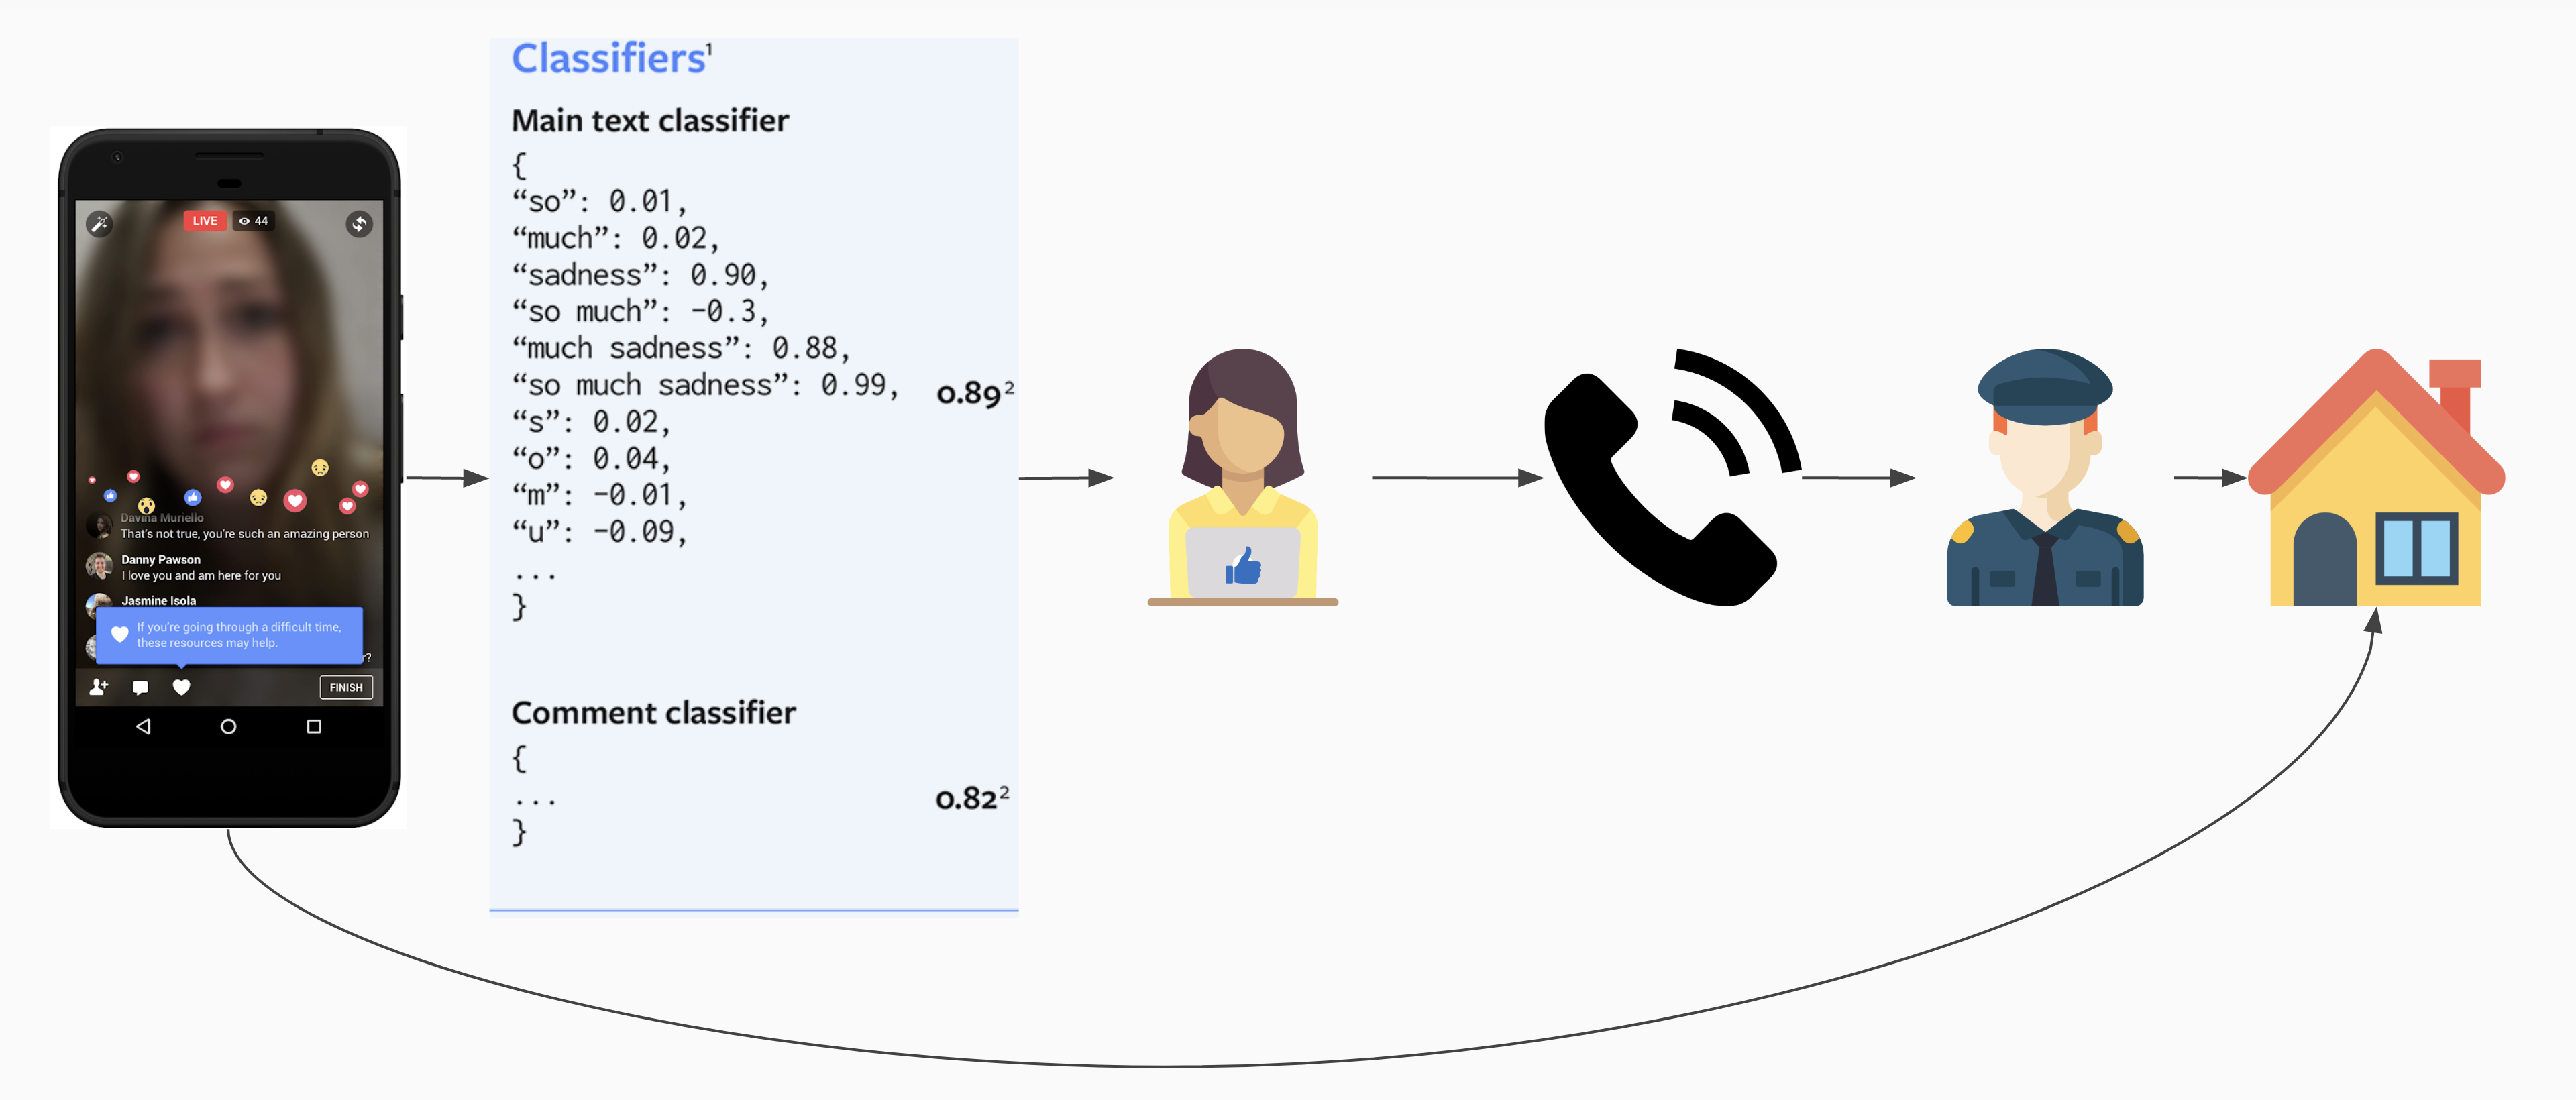
\includegraphics[width=\textwidth]{potentially-problematic-reporting-flow}
    \centering
    \small
    \textit{Can you anticipate problems with this reporting flow?}
\end{frame}

\begin{frame}{A Closer Look at Text and Comment Classifiers (Facebook)}
    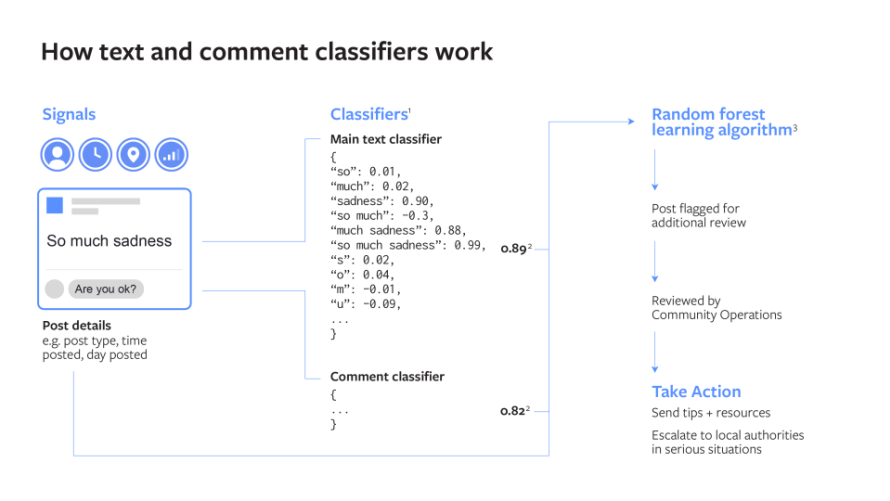
\includegraphics[width=\textwidth]{text-and-comment-classifiers}
    \small
    \href{https://about.fb.com/news/2018/09/inside-feed-suicide-prevention-and-ai/}{Source: Facebook Newsroom}
\end{frame}

\begin{frame}{ML for Detecting Suicidal Ideation (An Example)}
    \begin{columns}
        \column{0.4\textwidth}
            \small
            Can you apply ML to identify suicide ideation?
            \begin{itemize}
                \small
                \item Study consisted of 134 voluntary participants
                \item 8 false positives, 3 false negatives
                \item \textit{Twitter data only}
            \end{itemize}
            \vspace{0.05\textheight}
            \tiny
            \textit{“RESULTS: Our findings show that people who are at high suicidal risk can be easily differentiated from those who are not by machine learning algorithms, which accurately identify the clinically significant suicidal rate in 92\% of cases (sensitivity: 53\%, specificity: 97\%, positive predictive value: 75\%, negative predictive value: 93\%).”}
        \column{0.6\textwidth}
            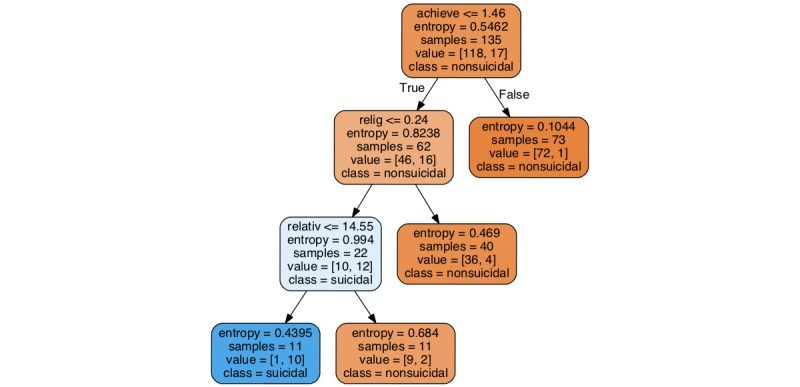
\includegraphics[width=\textwidth]{ml-identification}
    \end{columns}
    \vspace{0.02\textheight}
    \tiny
    Braithwaite, Scott R et al. “Validating Machine Learning Algorithms for Twitter Data Against Established Measures of Suicidality.” JMIR mental health vol. 3,2 e21. 16 May. 2016, doi:10.2196/mental.4822
\end{frame}

\section{Challenges and Considerations}

\begin{frame}{Criticism from Recovery Communities}
    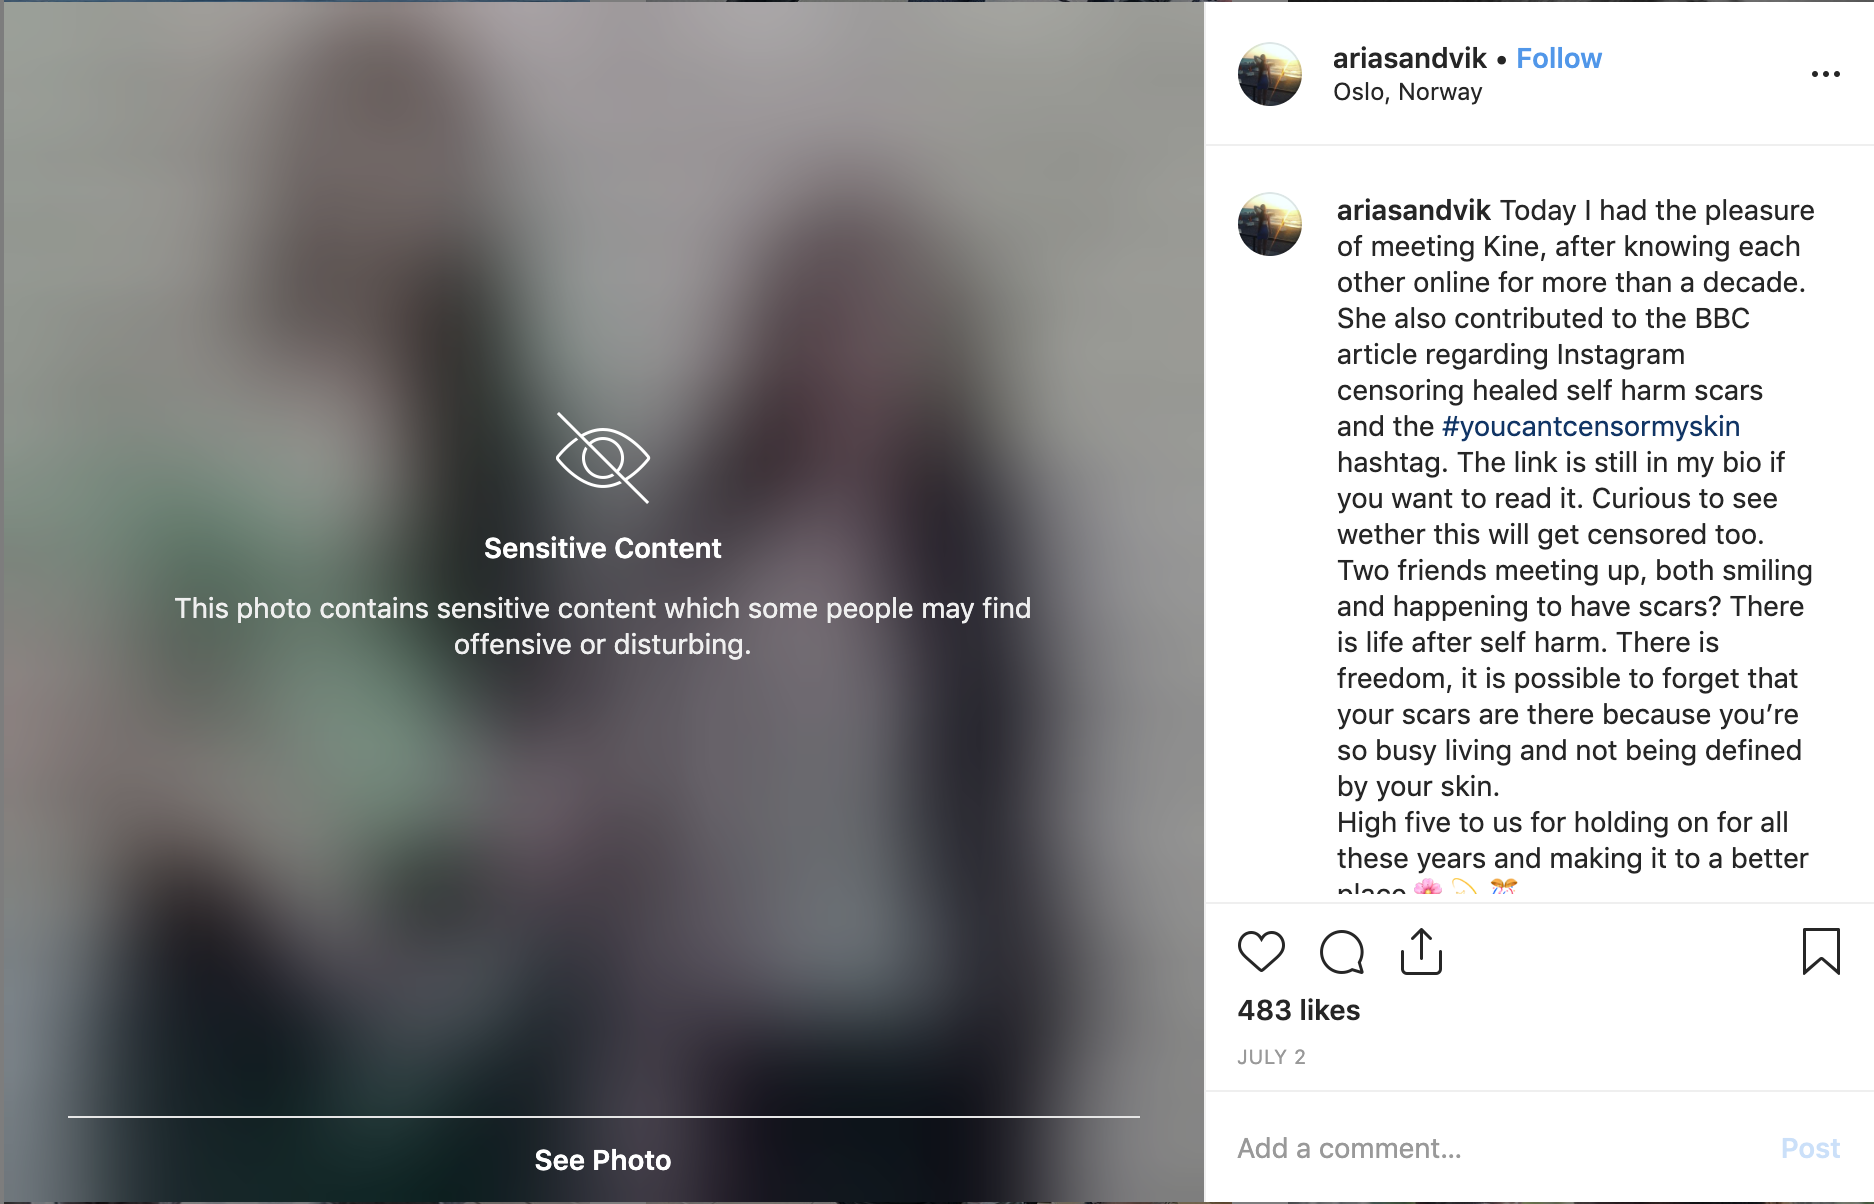
\includegraphics[width=\textwidth]{recovery-community-criticism-1}
\end{frame}

\begin{frame}{Criticism from Recovery Communities}
    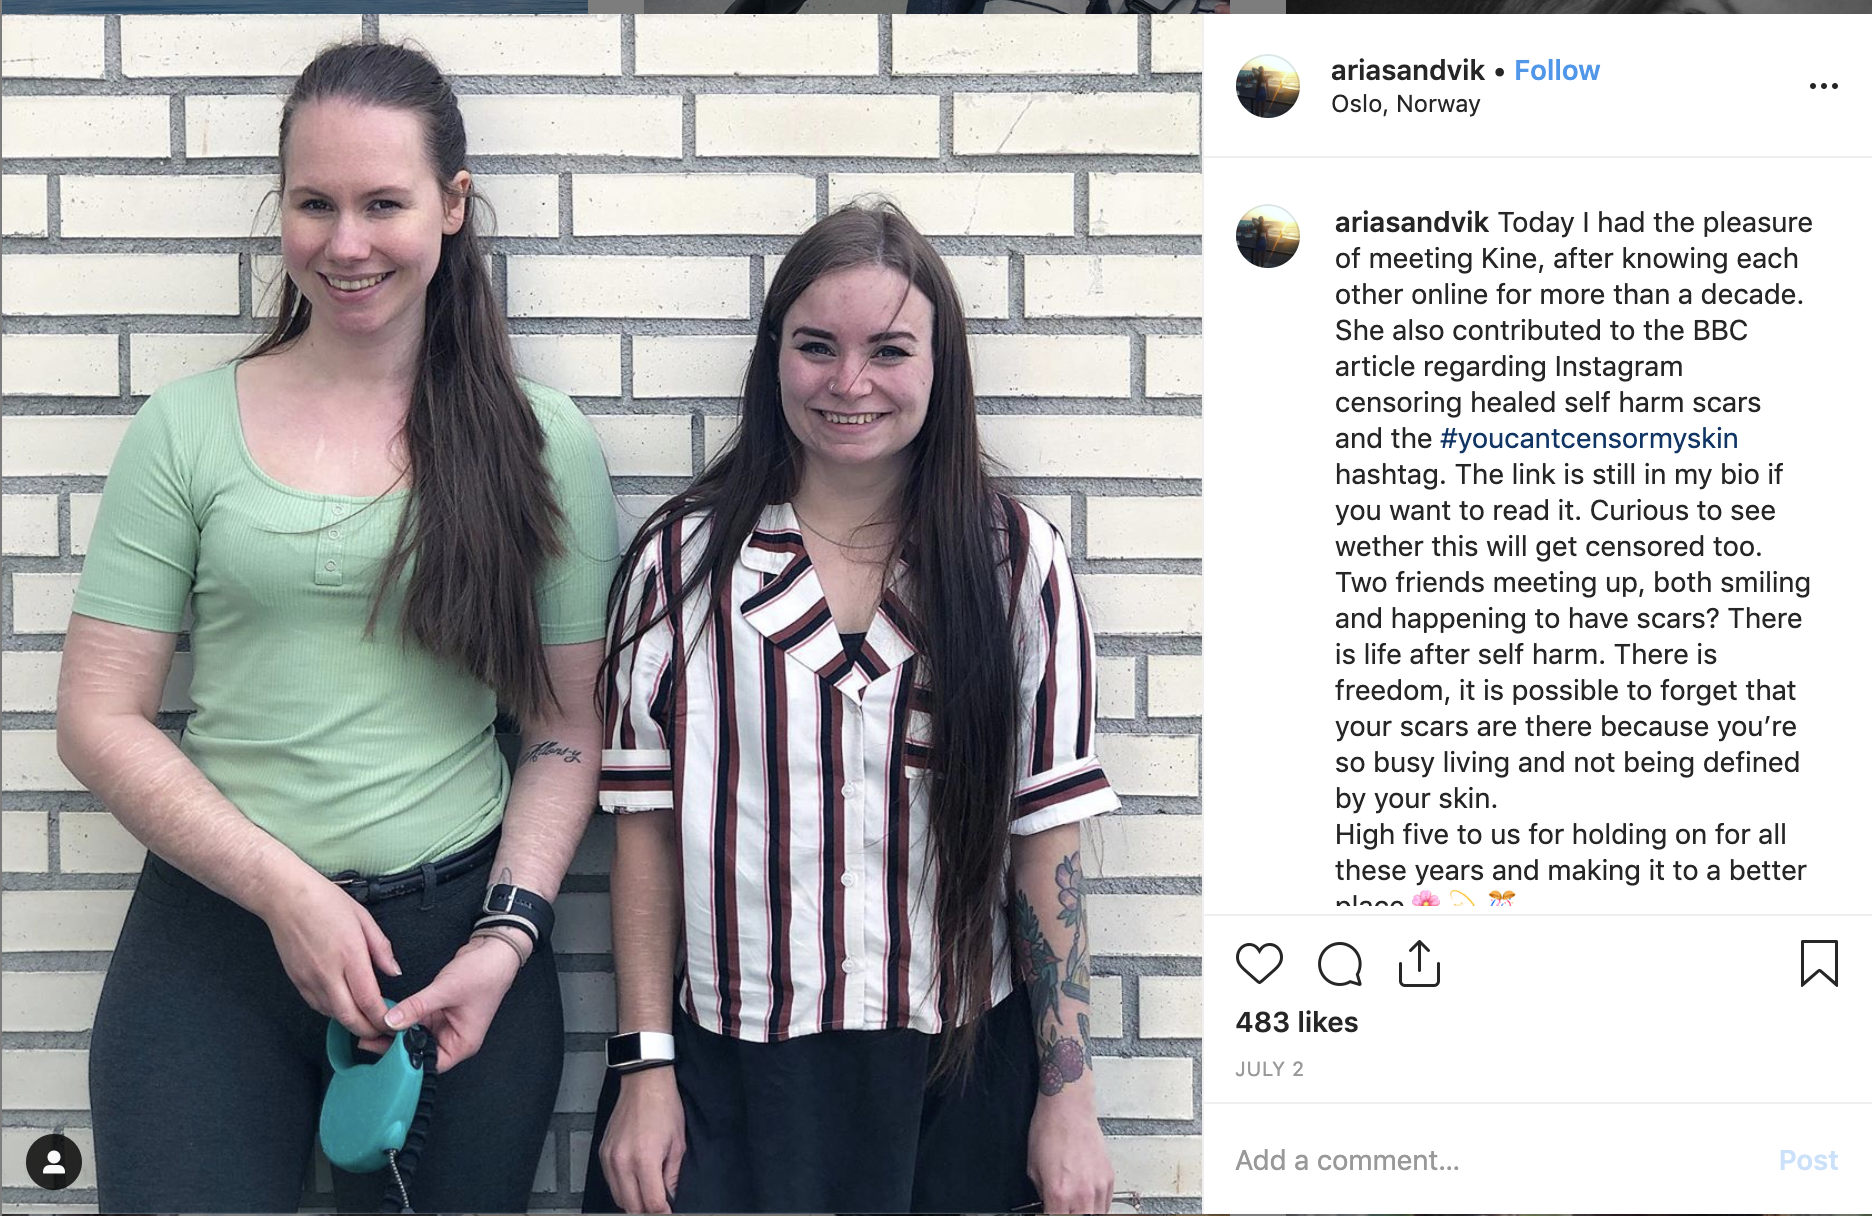
\includegraphics[width=\textwidth]{recovery-community-criticism-2}
\end{frame}

\begin{frame}{Criticism from Recovery Communities}
    
\includegraphics[width=\textwidth]{recovery-community-criticism-3}
\end{frame}

\begin{frame}{Emerging Challenges}
    \begin{itemize}
        \item How about voice assistants? Google Assistant in 2017:
    \end{itemize}
    \vspace{0.01\textheight}
    \begin{columns}
        \column{0.5\textwidth}
            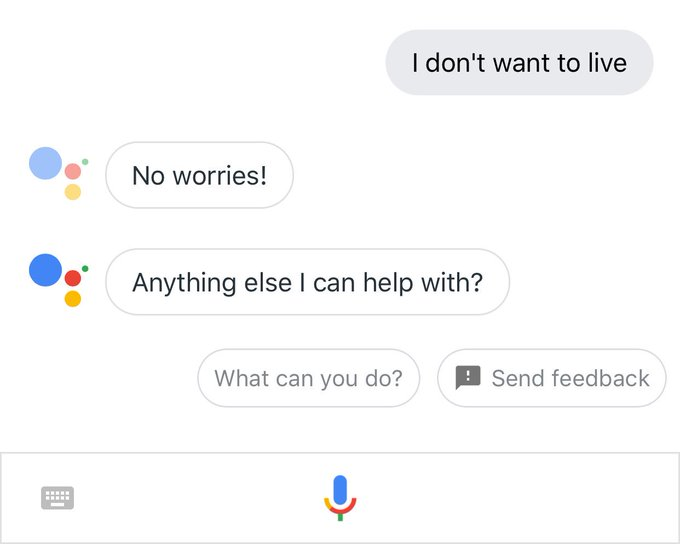
\includegraphics[width=\textwidth]{google-assistant-2017-text}
            \tiny
            \url{https://twitter.com/ManeeshJuneja/status/922390506172280832}
        \column{0.5\textwidth}
            \href{https://drive.google.com/file/d/1c-85YMp_Q-77P-phGZ_S-EI1lzDLfrv-/view}{
\includegraphics[width=\textwidth]{google-assistant-video}}
    \end{columns}
\end{frame}

\begin{frame}{Voice Assistants: 2022 - Prompted with “I don’t want to live”}%TODO need upload link to videos on YT/Drive
    \begin{columns}
        \column{0.25\textwidth}
            \href{}{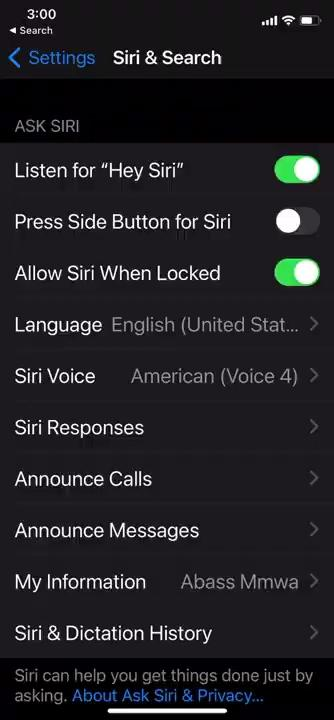
\includegraphics[width=\textwidth]{2022-response-siri}}
        \column{0.25\textwidth}
            \href{}{
\includegraphics[width=\textwidth]{2022-response-google-assistant}}
    \end{columns}
\end{frame}

\begin{frame}{Global Accessibility}
    \centering
    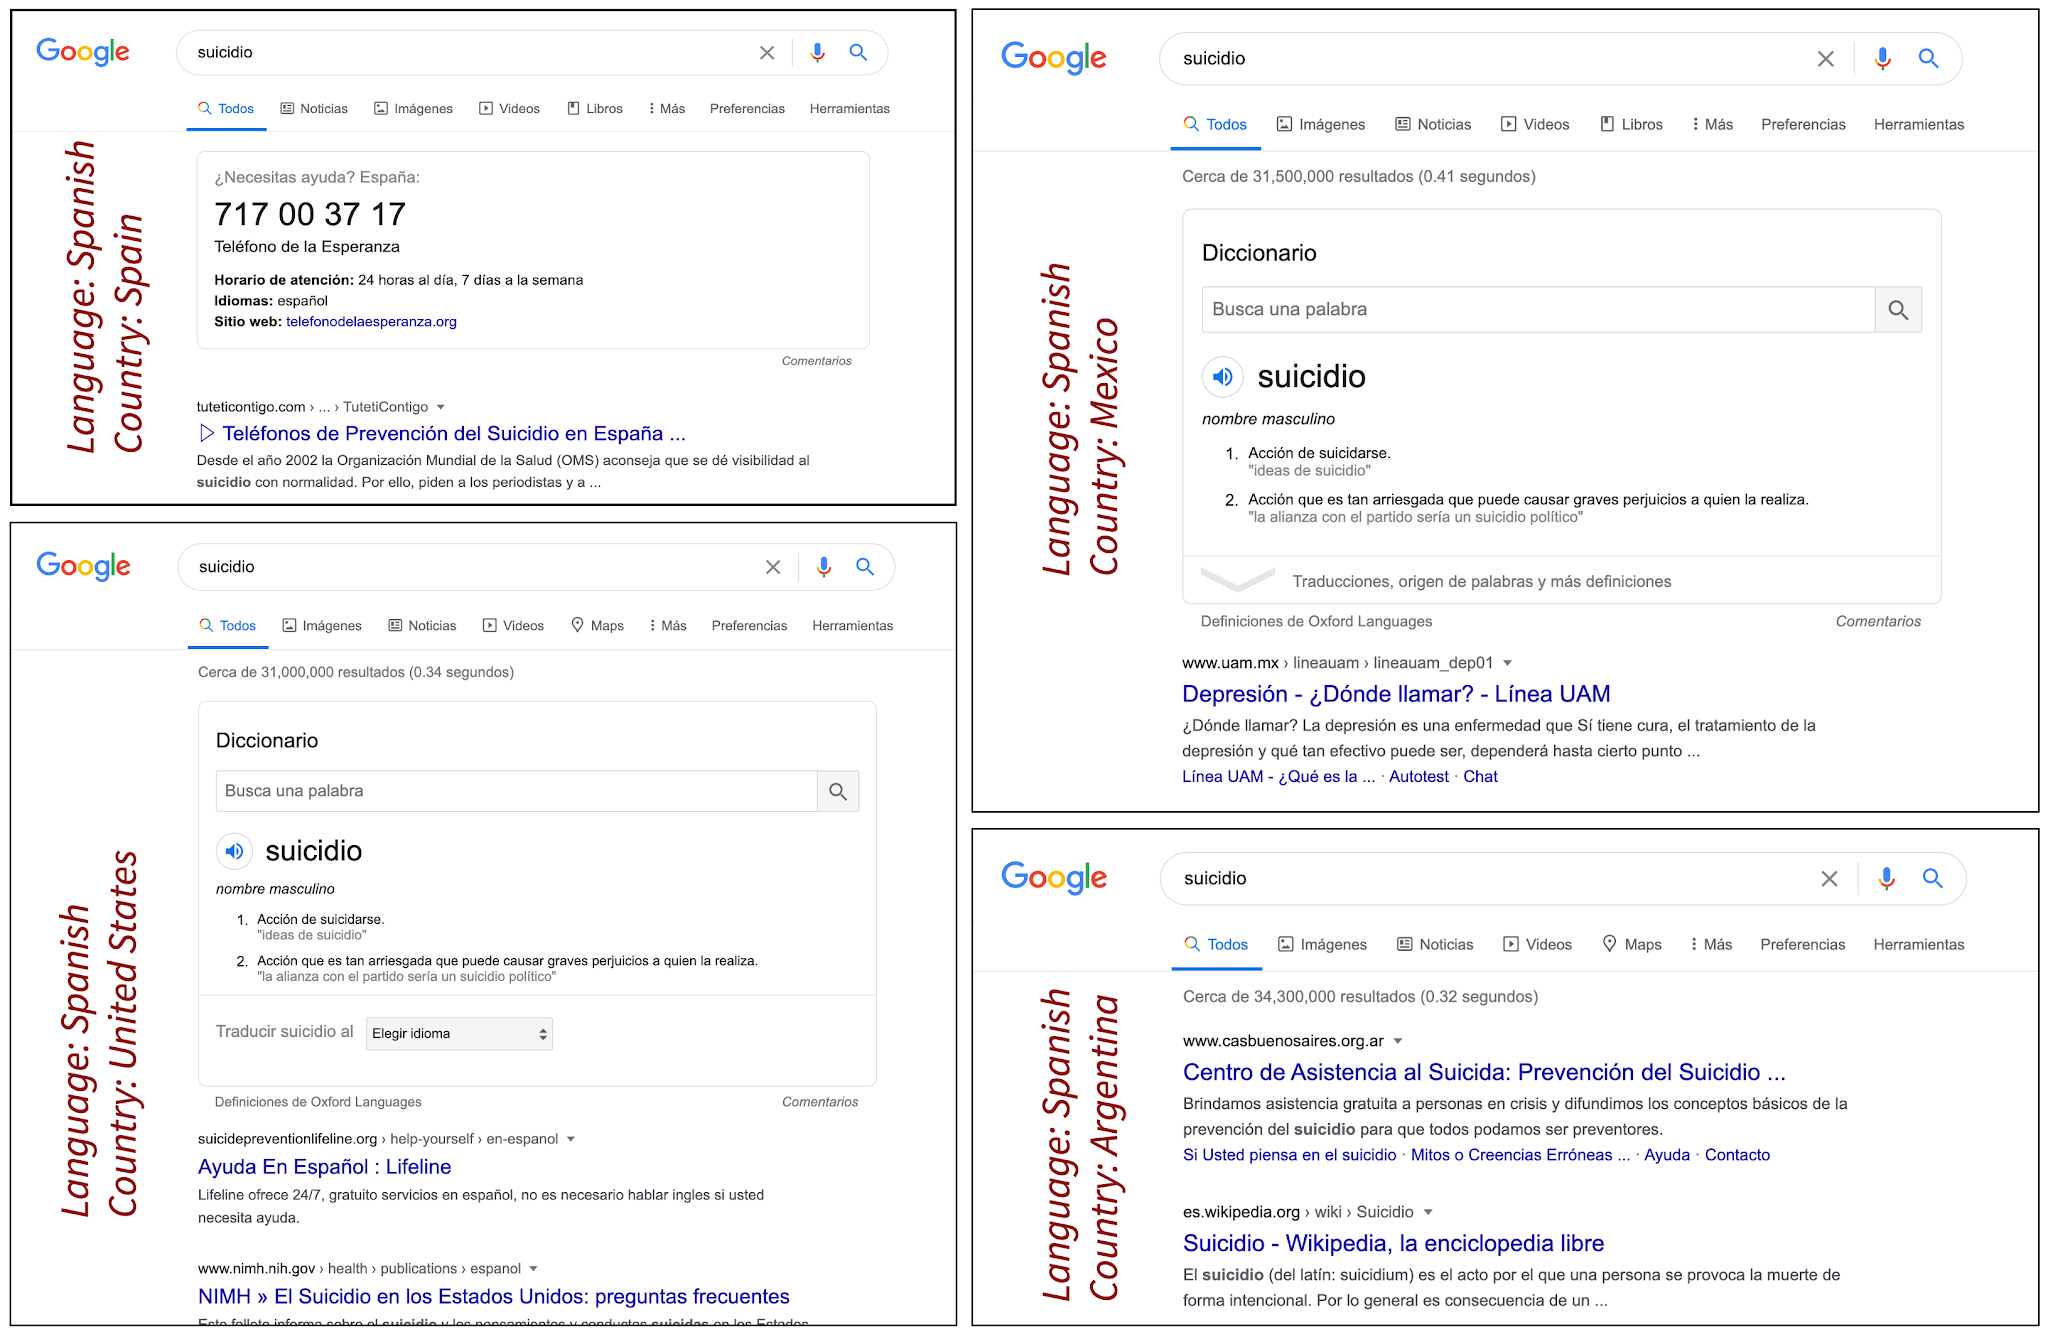
\includegraphics[width=\textwidth]{global-accessibility}
\end{frame}

\begin{frame}{Global Accessibility}
    Considerations:
    \begin{itemize}
        \item Is there a trustworthy civil society partner with the capacity to receive platform referrals?
        \begin{itemize}
            \item In the absence of such a partner, are resources from other organizations relevant and applicable?
        \end{itemize}
        \item Are there different search terms or contextual linguistic considerations?
        \item Are users mixing search terms from multiple languages to enhance discoverability or skirt filters?
        \item Do local laws regulate suicide and self-harm differently? Could referring an incident to the police result in an arrest rather than a wellness check?
        \item Do local privacy laws prevent or limit the application of classifiers?
    \end{itemize}
\end{frame}

\begin{frame}{User Feedback}
    \begin{columns}
        \column{0.4\textwidth}
            Are these responses working?\\~\\
            Are they too impersonal?\\~\\
            What is the optimal response?\\~\\
            Are there negative externalities from these actions?
        \column{0.6\textwidth}
            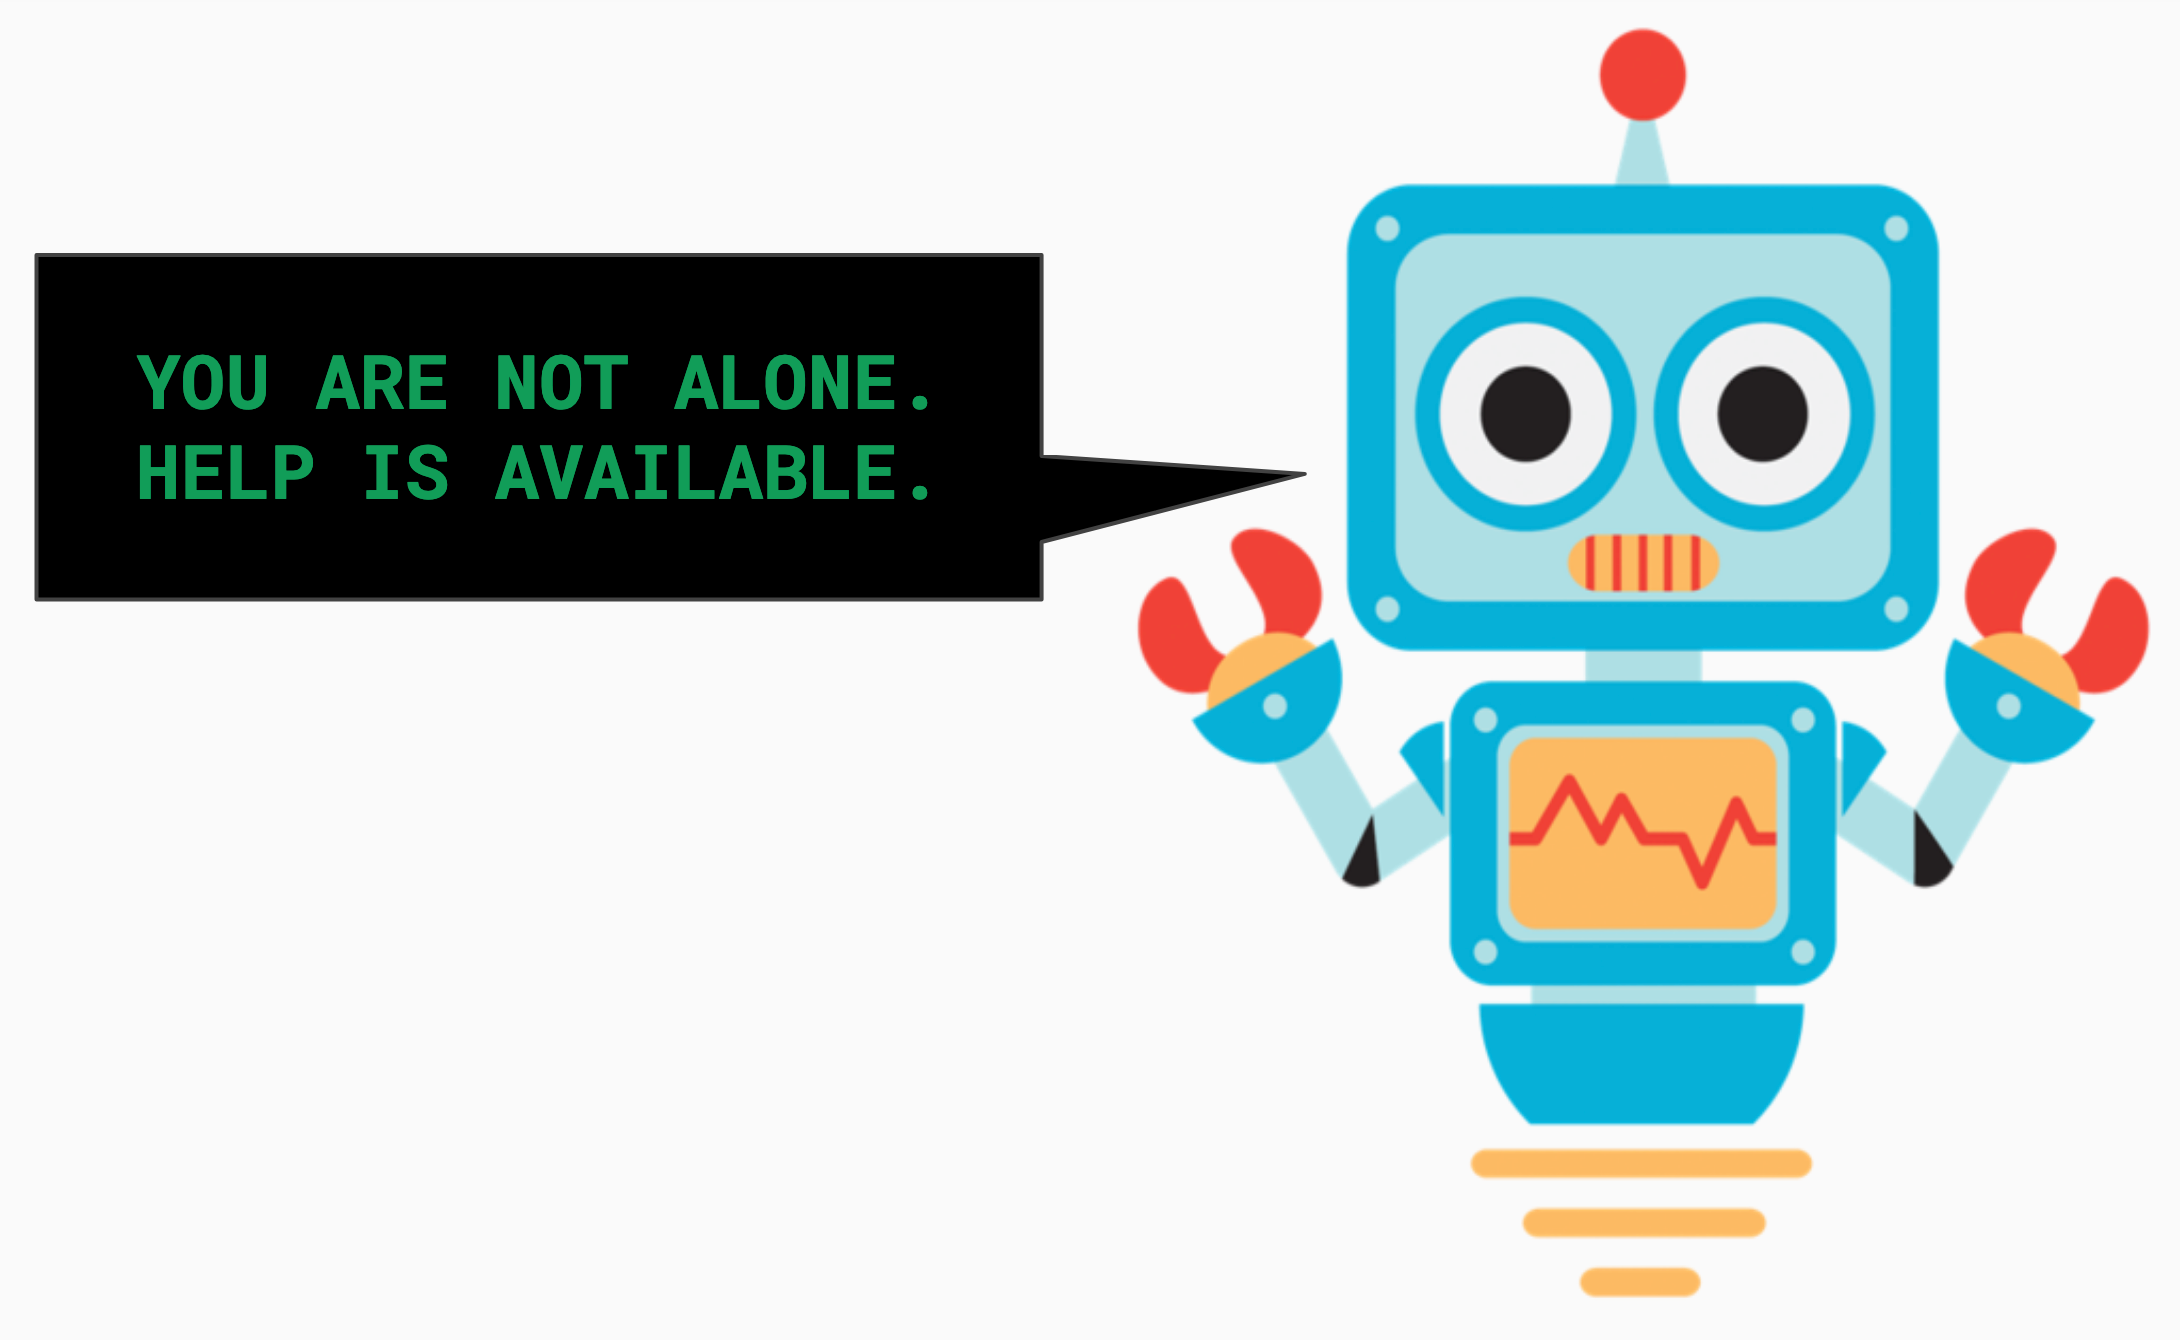
\includegraphics[width=\textwidth]{cute-robot}
    \end{columns}
\end{frame}

\begin{frame}{These Issues Aren't Isolated to Adolescent Girls}
    \small
    Suicide is the second leading cause of death for individuals between 15-34.\\
    The highest \underline{\textit{rate}} of suicide is among older men.
    \begin{columns}
        \column{0.4\textwidth}
            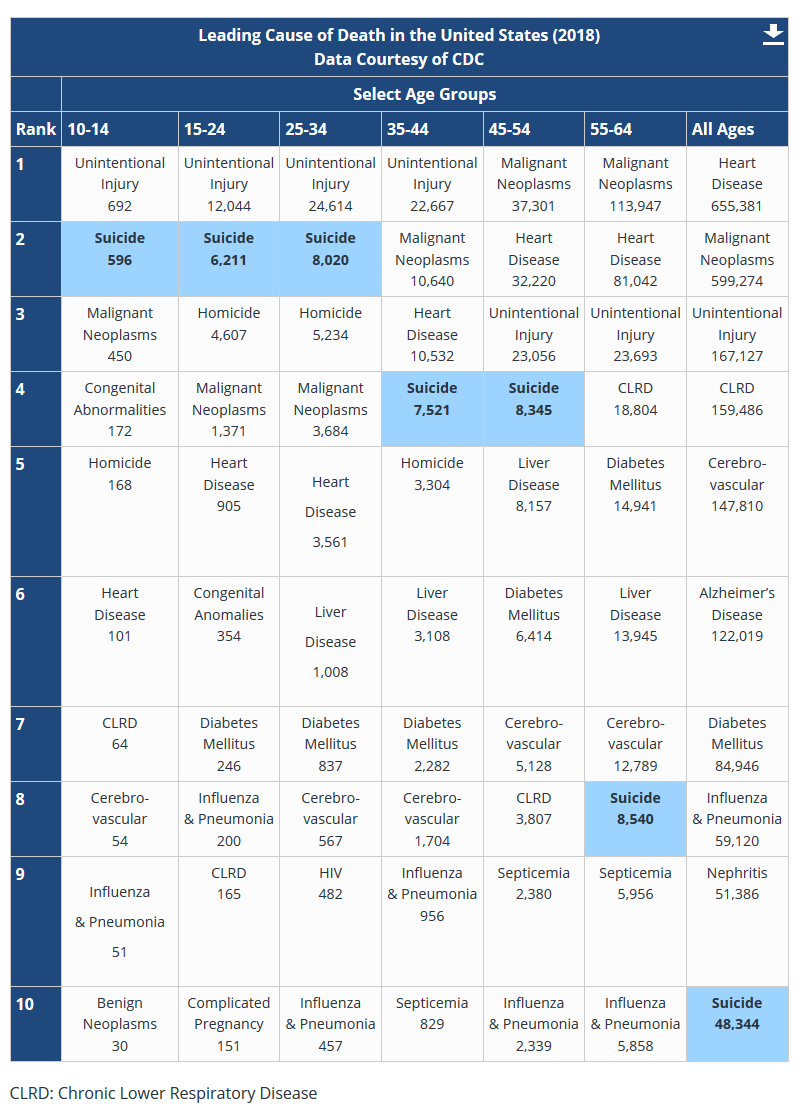
\includegraphics[width=\textwidth]{leading-causes-of-death-suicide-2018}
        \column{0.6\textwidth}
            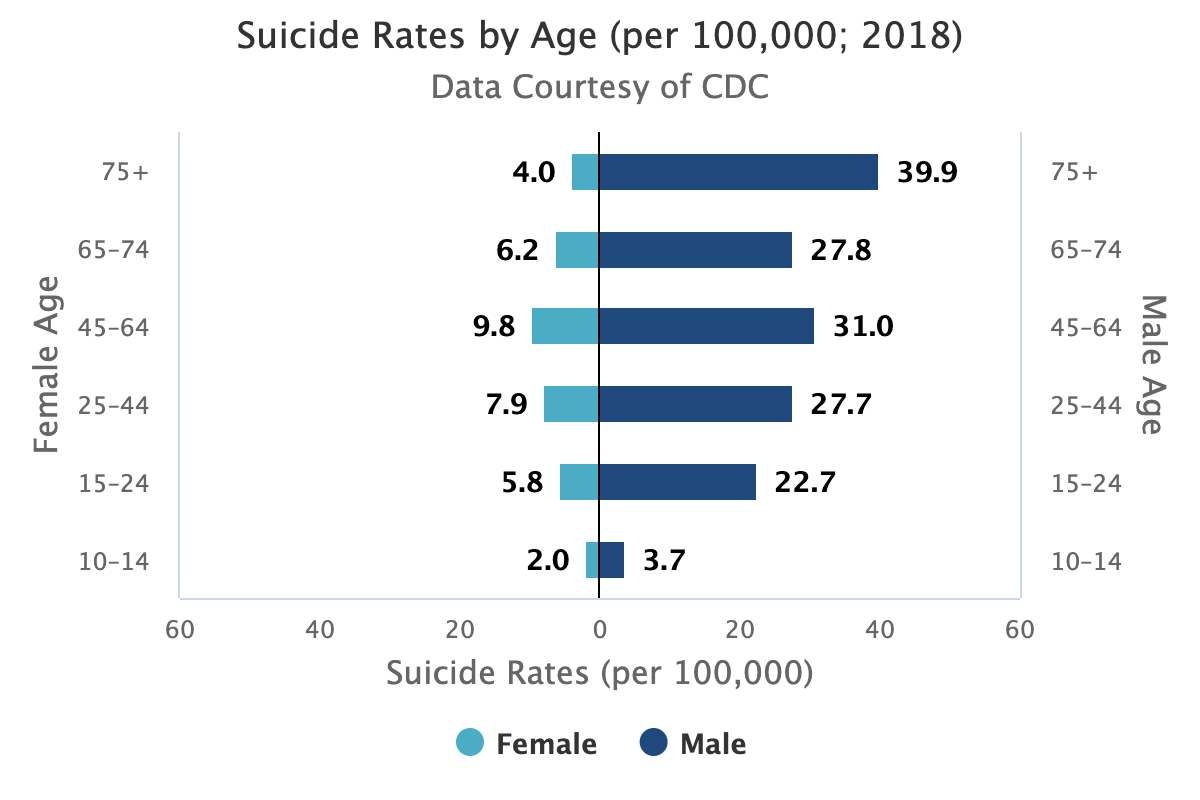
\includegraphics[width=\textwidth]{suicide-rates-by-age}
    \end{columns}
\end{frame}

\section{Contagion Effect}

\begin{frame}{Contagion Effect}
    \large
    Exposure to suicide-related content increases the likelihood of an individual engaging in suicidal behavior; this is especially true when the deceased is a relatable person (i.e., a celebrity or peer)
\end{frame}

\begin{frame}{"13 Reasons Why"}
    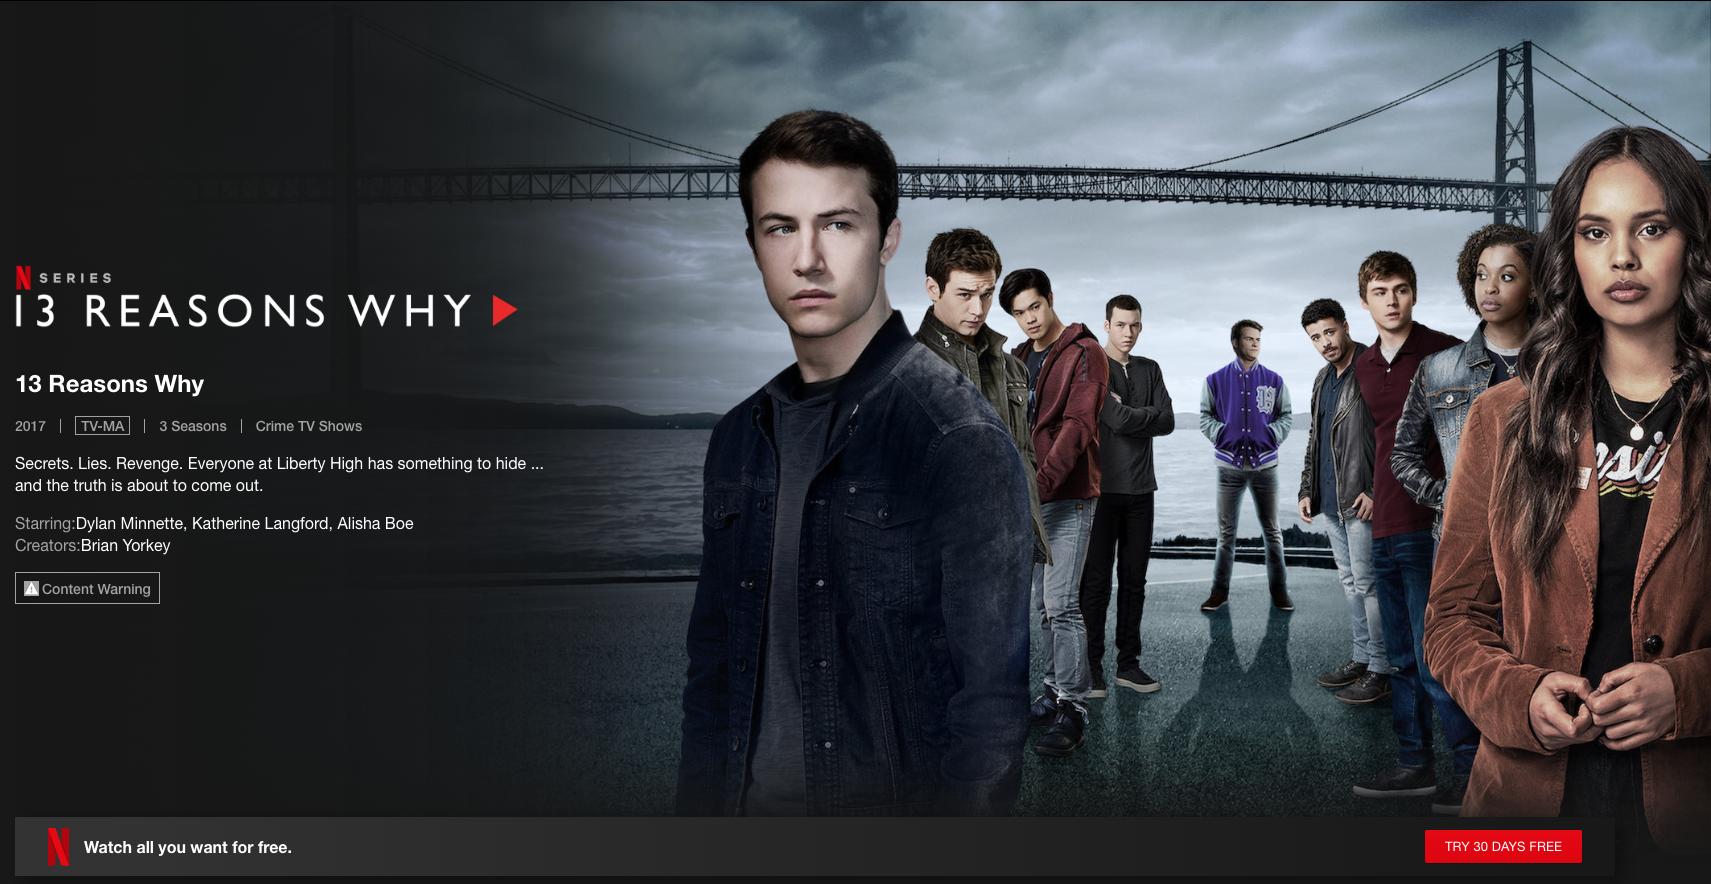
\includegraphics[width=\textwidth]{13-reasons-why-netflix}
\end{frame}

\begin{frame}{"13 Reasons Why"}
    \begin{itemize}
        \item Show criticized for graphic presentation of suicide, which goes against best practice for portraying suicide
        \item Led to an increase in suicide
    \end{itemize}
    
\includegraphics[width=\textwidth]{13-reasons-why-study-1}
    
\includegraphics[width=\textwidth]{13-reasons-why-study-2}
    
\includegraphics[width=\textwidth]{13-reasons-why-study-3}
\end{frame}

\begin{frame}{"13 Reasons Why"}
    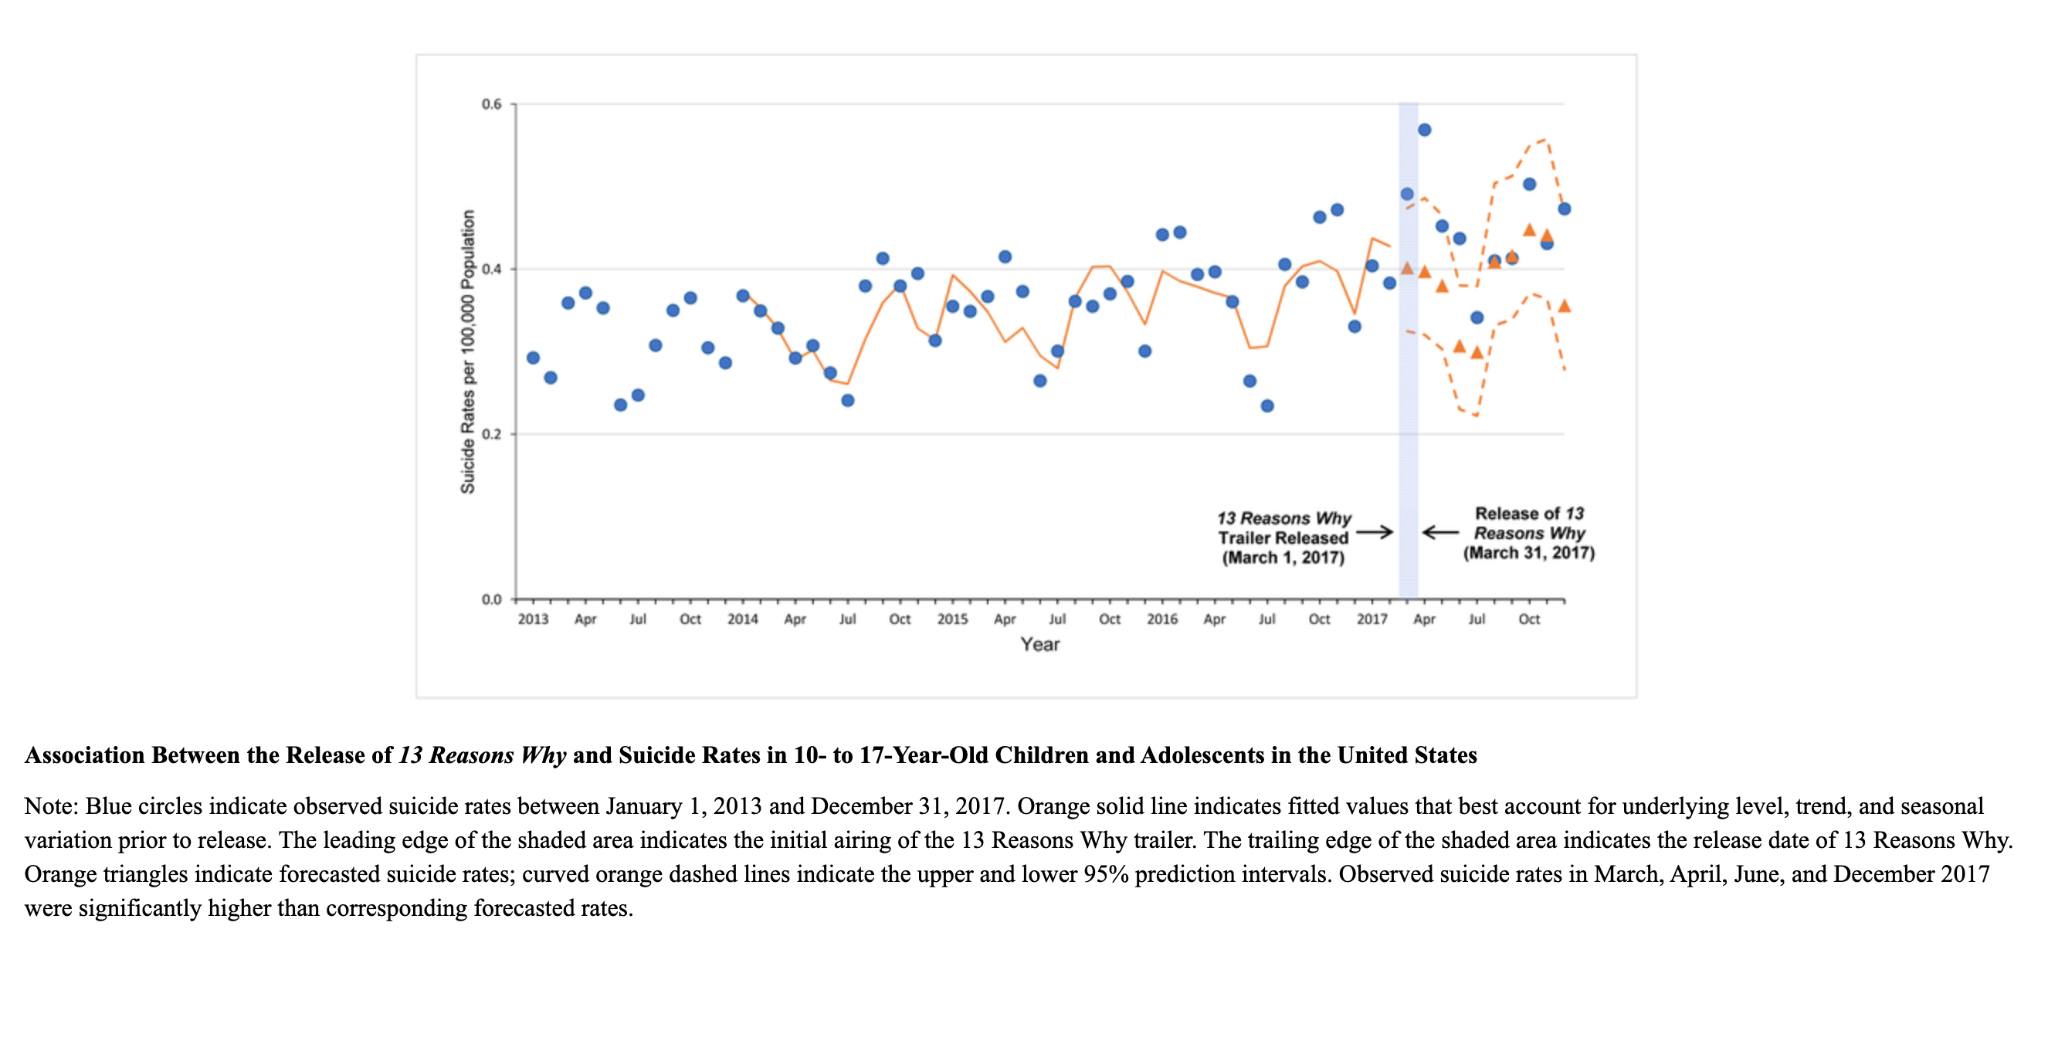
\includegraphics[width=\textwidth]{13-reasons-why-impact-on-adolescent-suicides}
\end{frame}

\begin{frame}{Effect is More Pronounced for Boys}
    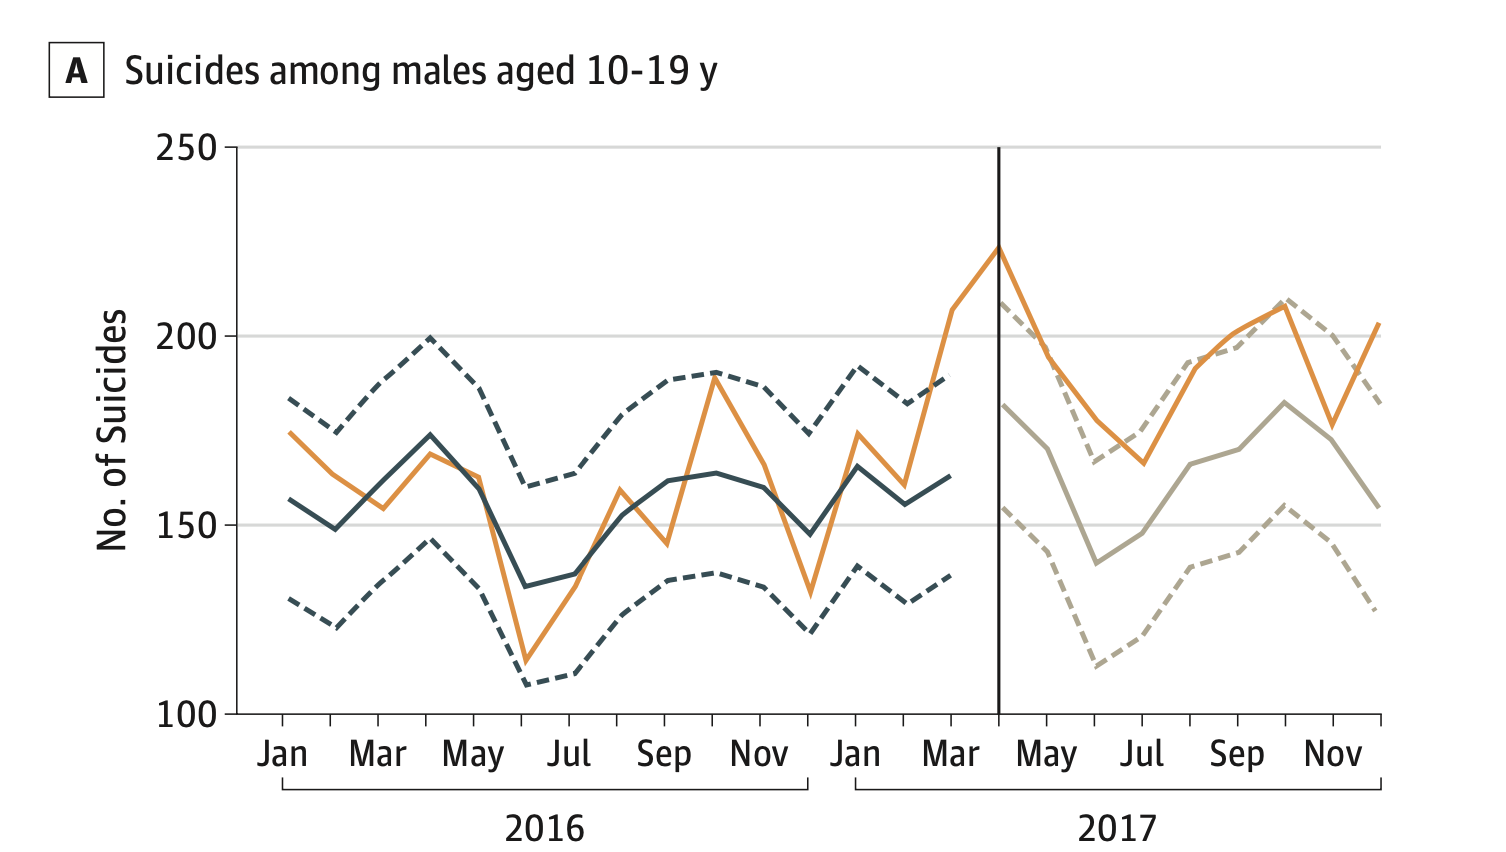
\includegraphics[width=\textwidth]{13-reasons-why-stronger-impact-on-boys}
\end{frame}

\begin{frame}{Celebrity Deaths and the Contagion Effect}
    \centering
    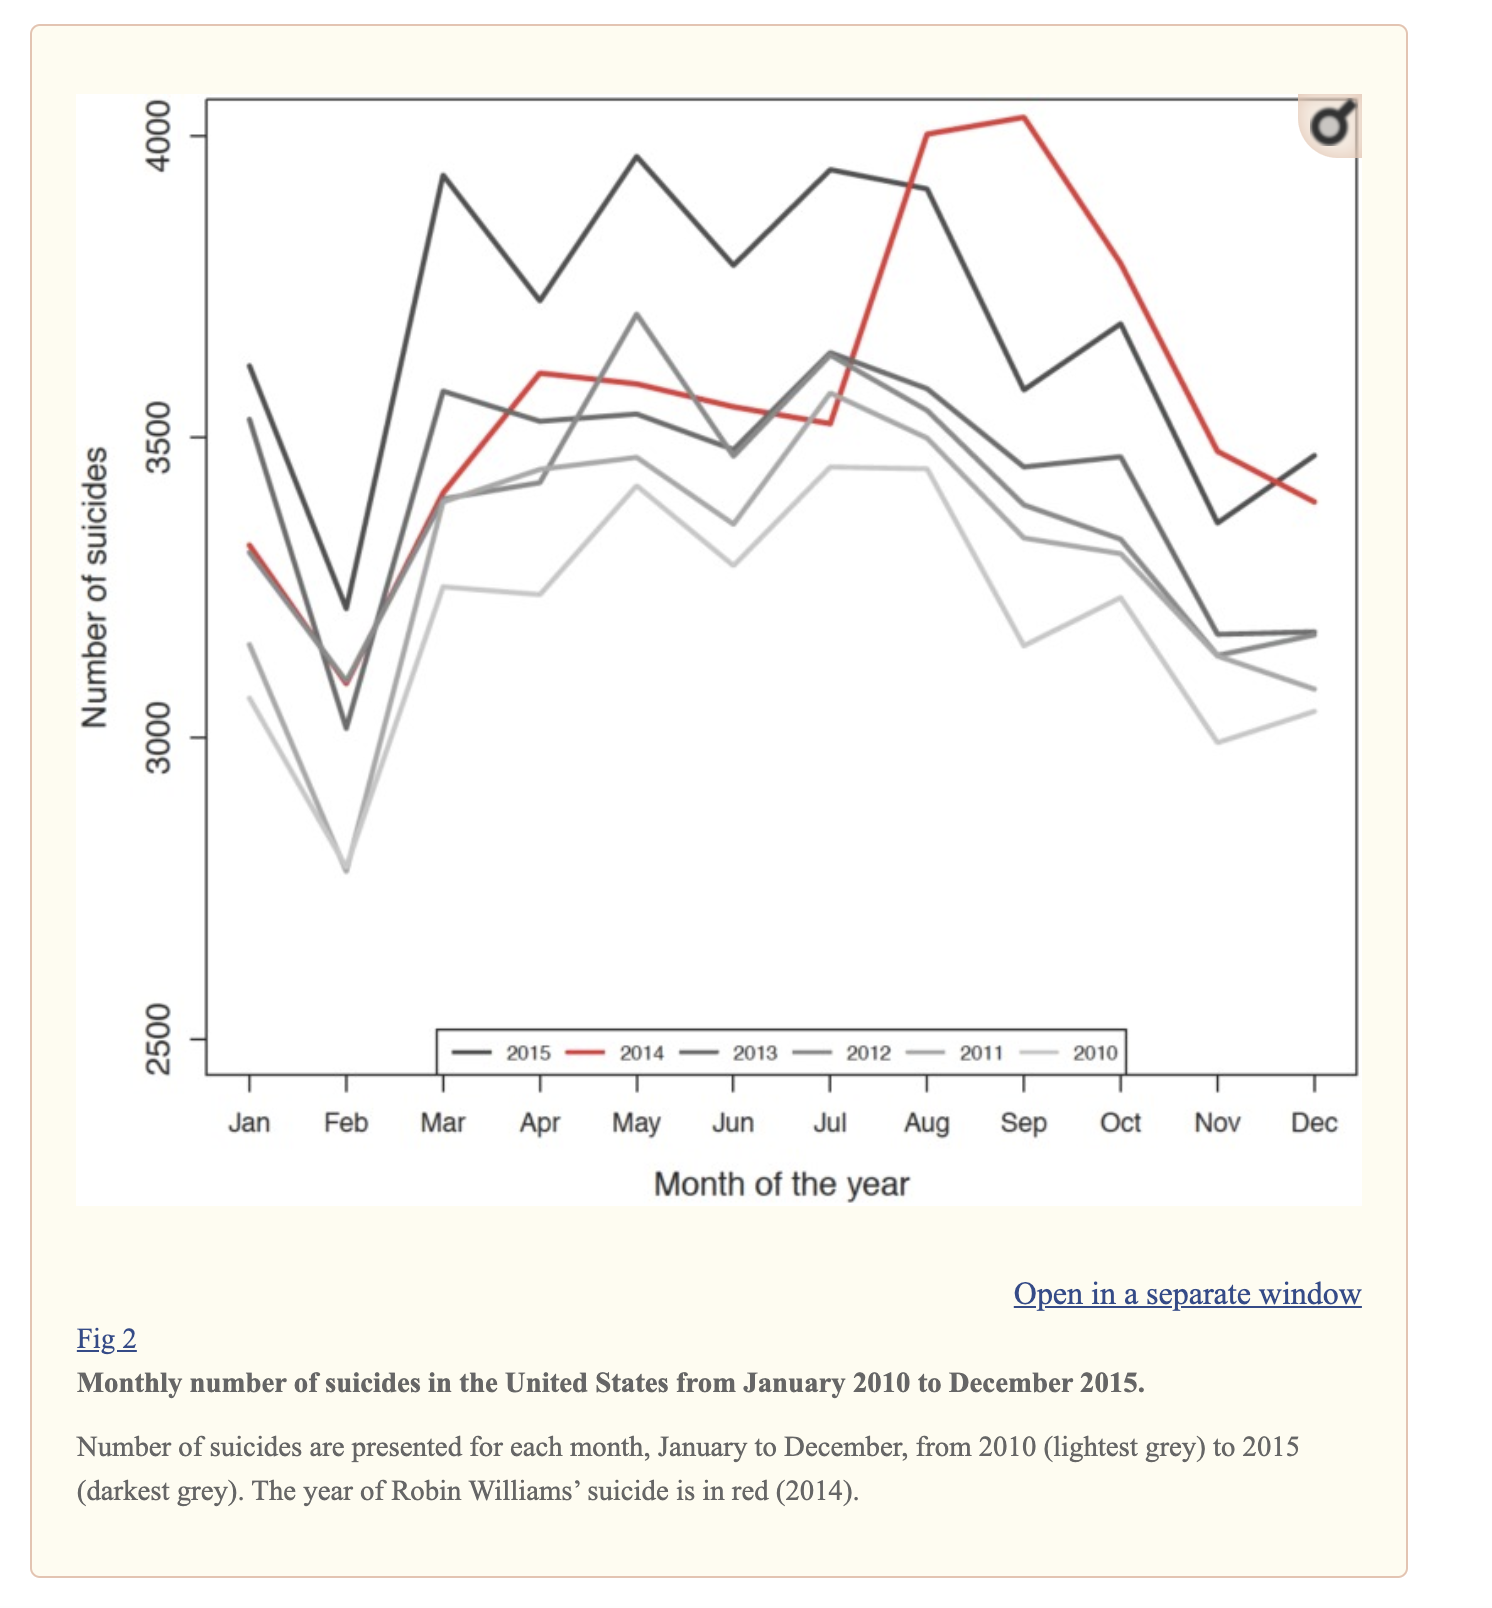
\includegraphics[height=0.88\textheight]{celebrity-deaths-contagion-effect}
\end{frame}

\section{Food for Thought}

\begin{frame}{Food for Thought}
    \begin{itemize}
        \item What are platforms responsibilities in preventing self-harm?
        \item This is a wider conversation that cannot be handled alone by technical interventions
        \item What is the social sector infrastructure?
        \item There is no silver bullet
        \item Technology companies are not qualified to \textit{drive} the solution but they can \textit{support} the solution
        \item Consult with experts
    \end{itemize}
\end{frame}

\end{document}